\chapter{File and Filesystem Programming}

% https://tldp.org/LDP/intro-linux/html/sect_03_04.html - chmod / file masks etc this stuff should go in the programming chapter or somewhere else

Before diving into the Linux kernel to understand how files and filesystems are accessed and how filesystems operate internally, it's best to look at what's happening in user space by understanding how applications access files. Much of what the kernel does is to satisfy a set of system calls (functions in the kernel that programs access). A process, which is the running instantiation of an executable program, either access this set of system calls directly or uses a set of library functions which in turn use the system call interface.

This chapter explores all the different ways that applications can access files from basic \cf{read(2)} and \cf{write(2)} system calls to the standard I/O library to asynchronous I/O and less-used features such as extended attributes. 

\section{Programming Standards and Portability}

Around the time of my last book, we were still living in a world of multiple different UNIX and UNIX-variants of which Linux was one key player. Over the years, there have been several standards bodies created to develop a common set of programming interfaces that each of the operating system vendors diligently worked to adopt to make the life of application developers much easier. I remember working with several dedicated people attending standards meetings of one form or another, implementing these changes and ensuring that the interfaces adhered to the standard by using a common set of test suites.

With Linux and Windows now dominating approximately 90\% of the server operating system market, there are only really two platforms now to consider and a relatively small number of Linux distributions covering all Linux installed systems. Of course if we consider smart phones and tablets, that means Android (also Linux based) and iOS. Although these applications are very different from those in the server world, application portability is still important. Wherever possible, you should use standard interfaces. Having a high-level of portability across not just Windows and Linux but Apple OS/X and the various BSD operating systems is still a smart choice.

It's beyond the scope of this book to discuss all the issues around source code portability but I wanted to at least highlight the different standards that are our there to make you aware before you delve into writing a complex application. Think about where that application may end up in future even if operating system portability isn't a goal initially. You will want to think carefully about the toolchain that you'll use as part of the development process. 

The Linux manual pages indicate which standard the functions they describe adhere to. Let's take three examples. Starting with the \cf{write(2)} system call:

\begin{lstlisting}
CONFORMING TO
	   SVr4, 4.3BSD, POSIX.1-2001.
\end{lstlisting}

\noindent 
For the \cf{printf(3)} library function:

\begin{lstlisting}
CONFORMING TO
	fprintf(), printf(), sprintf(), vprintf(), vfprintf(),
	vsprintf(): POSIX.1-2001, POSIX.1-2008, C89, C99.

	snprintf(), vsnprintf(): POSIX.1-2001 & 2008, C99.

	dprintf() and vdprintf() functions were originally GNU
	extensions and were later standardized in POSIX.1-2008.
\end{lstlisting}

\noindent
The \cf{getenv(3)} manual page is a little different. It also describes \cf{secure\_getenv()} which it states "\textit{is a GNU extension}":

\begin{lstlisting}
CONFORMING TO
	getenv(): POSIX.1-2001, POSIX.1-2008, C89, C99, 
	          SVr4, 4.3BSD.

	secure_getenv() is a GNU extension.
\end{lstlisting}

\noindent 
This could mean that it's not portable across different operating systems so be careful of such extensions.

\subsection{What are all These Standards?}

There have been many attempts at standardization over the last few decades. Here are the prominent staandards and how they relate to Linux:

\begin{itemize}
	\item POSIX --- The Portable Operating System Interface (POSIX and pronounced \textit{pahz-icks}) 
		is a family of standards specified by IEEE. It defines both system- and user-level "\textit{Application 
		Programming Interfaces}" (APIs), along with command line shells and utility interfaces, for software 
		compatibility (portability) with variants of UNIX and other operating systems. 
	\item Single UNIX Specification (SUS) --- a standard that specifies programming interfaces for the C language, 
		a command-line shell, and user commands. Conformance with SUS allowed operating systems vendors
		to use the name 'UNIX" as part of their brand offering. What started out as \textit{Spec 1170}, a
		set of 1,170 commands/interfaces, the collection of all such interfaces would eventually become the Single Unix Specification.
		Very few Linux and BSD vendors/distributions have gone through certification and with the number of UNIX versions declining, 
		we are unlikely to see any more.
	\item C89 - C2x --- ANSI C - standards for the C programming language. As you can see from the manual pages
		of three functions above, many Linux functions state compliance. 
	\item Linux Standard Base (LSB) --- formed by the Linux Foundation, LSB was a joint project 
		comprising multiple Linux distributions with the goal to standardize Linux software system structure, 
		including the \textit{Filesystem Hierarchy Standard} used in the Linux kernel. LSB was based 
		on the POSIX specification, the Single UNIX Specification (SUS), and several other open standards, 
		but it also extended them in some areas.
\end{itemize}

\noindent
The first version of POSIX.1 was published in 1988 and the most recent in 2017. Prior to 1997, POSIX was split into several different sub-standards which I'm listing in full below to show how extensive the standard actually was. I recall working on an implementation of threads on an SVR4 UNIX subsystem on the Chorus microkernel while the standard was still being developed back in the early 1990s.

\begin{itemize}
	\item POSIX.1: Core Services (incorporates Standard ANSI C) 
		\begin{itemize}
			\item Process Creation and Control
			\item Signals
			\item Floating Point Exceptions
			\item Segmentation / Memory Violations
			\item Illegal Instructions
			\item Bus Errors
			\item Timers
			\item File and Directory Operations
			\item Pipes
			\item C Library (Standard C)
			\item I/O Port Interface and Control
			\item Process Triggers
		\end{itemize}
	\item POSIX.1b: Real-time extensions
		\begin{itemize}
			\item Priority Scheduling
			\item Real-Time Signals
			\item Clocks and Timers
			\item Semaphores
			\item Message Passing
			\item Shared Memory
			\item Asynchronous and Synchronous I/O
			\item Memory Locking Interface
		\end{itemize}
	\item POSIX.1c: Threads extensions
		\begin{itemize}
			\item Thread Creation, Control, and Cleanup
			\item Thread Scheduling
			\item Thread Synchronization
			\item Signal Handling	
		\end{itemize}
	\item POSIX.2: Shell and Utilities
		\begin{itemize}
			\item Command Interpreter
			\item Utility Programs
		\end{itemize}
\end{itemize}

\noindent
After the first version of POSIX in 1988, there have been several other enhanced versions namely, POSIX.1-2001, POSIX.1-2008 and the final version, POSIX.1-2017. There is a nice FAQ on POSIX by the OpenGroup here if you wish to read further:

\begin{table}[h]
\begin{tabular}{lcl}
\parbox[r]{0.5in}{ 
\includegraphics[scale=0.15]{figures/url.png}} & \parbox[l]{0.1in}{\arabic{urls}} & \parbox[l]{3in}{\cf{https://tinyurl.com/5bnxjrae}}
\end{tabular}
\end{table}
\stepcounter{urls}
% https://www.opengroup.org/austin/papers/posix_faq.html

\subsection{LSB --- Linux Standard Base}

The Linux Standard Base covered everything from standard libraries, commands and utilities that extended the POSIX standard, file system hierarchy layout, run levels, X Window System extensions, System V UNIX-style initialization scripts and others. Version 1.0 of LSB was released in 2001 and the last version (5.0) in 2015. There were 21 release versions of Linux certified for LSB 4.0 but considerably fewer for 4.1.

LSB has certainly had its critics over the years. Apparently LSB 3.0 was released with a big yawn and also had critics from the glibc team for which it created a lot of additional work. One of the original goals of LSB was for application compatibility allowing 3rd party developers to write-once, run-anywhere including binary and package levels. The goals were sound with Linux leaders not wanting Linux distributions to diverge as the various UNIX vendors had in the past. 

Nowadays, relatively few Linux distributions dominate the landscape which reduces the demands for something like LSB and proprietary vendors tend to target specific distributions based on demands from their customer base. But LSB was largely successful in that it brought Linux vendors together at a time that divergence was a real possibility.

At the time of writing, the \cf{lsb\_release(1)} command, which did display LSB version details, now just displays information specific to the Linux release. As an example, for Ubuntu:

\begin{lstlisting}
$ [*\bfseries lsb\_release -a*]
No LSB modules are available.
Distributor ID:	Ubuntu
Description:	Ubuntu 22.10
Release:	22.10
Codename:	kinetic
\end{lstlisting}

\section{Manual Pages}

All functions that can be used by an application that are provided by the operating system have a corresponding manual page which is more commonly referred to as a "\textit{manpage}". For programming interfaces, the manpage documents expected parameters, return values and header files that need to be included. There are also manpages for all of the Linux commands, file formats and so on. You can do a keyword search to find manpages that are relevant to the keyword that you supply. For example, let's search for write-related man pages.

Below is a subset of what is shown when searching for write-related functions and commands. There is a command called \cf{write} as indicated by \cf{(1)} and the \cf{write} system call as indicated by \cf{(2)}.

\begin{lstlisting}
$ [*\bfseries man -k write*]
aio_write (3)        - asynchronous write
fwrite (3)           - binary stream input/output
pwritev (2)          - read or write data into multiple buffers
write (1)            - send a message to another user
write (2)            - write to a file descriptor
...
\end{lstlisting}

\noindent
What do the numbers in parenthesis mean? The UNIX (and now Linux) manual pages are divided into different sections. The section for each manpage is shown above in parenthesis. To see the list of available sections, you can run "\cf{man man}". Here are the nine sections for Linux:

\begin{lstlisting}
1   Executable programs or shell commands
2   System calls (functions provided by the kernel)
3   Library calls (functions within program libraries)
4   Special files (usually found in /dev)
5   File formats and conventions, e.g. /etc/passwd
6   Games
7   Miscellaneous (including macro packages and conventions),
	e.g. man(7), groff(7), man-pages(7)
8   System administration commands (usually only for root)
9   Kernel routines [Non standard]
\end{lstlisting}

\noindent
If you want to display the man page for the \cf{write()} system call, run "\cf{man 2 write}". If you want to see the "\cf{printf()}" manpage run "\cf{man printf(3c)}". And if you're unsure which section you need, use the "\cf{-k}" option. 

I have on occasion run into issues when trying to view manpages, specifically those related to programming. For example, if you see an error when running "\cf{man 2 open}" you need to install the development manpages as follows:

\begin{lstlisting}
$ [*\bfseries {sudo apt install manpages-dev*]
\end{lstlisting}

\noindent
There is a wealth of information in the Linux manpages. If you don't have a running system at hand, just enter "\cf{write(2)}" in your favorite search engine and you'll be able to view it online.

\section{System Calls vs Library Functions -- an Overview}

A software library is just a collection of source code functions and variables that are combined together into a single \textit{library file}. The library can't run by itself. When user programs are built, the source code is first compiled then it is \textit{linked} with one or more libraries to make an executable or binary.

When writing applications you will likely use a number of different library functions. Just take the first program that people usually write in C (or most other languages):

\begin{lstlisting}
#include <stdio.h>

int 
main()
{
	printf("Hello world!\n");
}
\end{lstlisting}

\noindent
The program can be compiled as follows to get an executable:

\begin{lstlisting}
$ [*\bfseries cc hello\_world.c -o hello\_world*]
\end{lstlisting}

\noindent
or "\cf{make hello\_world}" will achieve the same result. In this program we use a single library function called \cf{printf(3)} that is contained in what is known as the \textit{standard C library} (see \cf{libc7} for more information). To see what libraries our executable program is linked with, we can use the \cf{ldd(1)} command as follows:

\begin{lstlisting}
$ [*\bfseries ldd hello\_world*]
linux-vdso.so.1 (0x0000ffffb4e83000)
libc.so.6 => 
/lib/aarch64-linux-gnu/libc.so.6 (0x0000ffffb4c70000)
/lib/ld-linux-aarch64.so.1 (0x0000ffffb4e46000)
\end{lstlisting}

If library functions are just functions packaged together, what is the difference between a library function and a system call? When writing applications you use library functions which may perform the required function by themselves or they may call into the Linux kernel for services. For a simple program such as the one below, you may unaware of difference between one function type and another (error checking excluded for simplicity):

\begin{lstlisting}
#include <fcntl.h>
#include <stdio.h>
#include <unistd.h>
#include <string.h>

int
main()
{
    char buf[64];
    int  fd;

    fd = [*\bfseries open*]("msg", O_CREAT | O_WRONLY);
    [*\bfseries sprintf*](buf, "hello world -> fd = %d\n", fd);
    [*\bfseries write*](fd, buf, [*\bfseries strlen(buf)*]);
}

\end{lstlisting}

\noindent
There are four different functions called two of which are system calls (\cf{open} and \cf{write}) and two which are not. As programmers gain experience they will generally know which functions are system calls and which are not without having to check the manpages. Later sections in the book will describe system call handling for file and filesystem-related functions in detail.

\section{Error Handling with \cf{errno}}

As the \cf{errno(3)} manpage says:

\begin{quote}
\textit{The  <errno.h> header file defines the integer variable errno, which is set by system calls and some library functions in the event of an error to indicate what went wrong.}
\end{quote}

\noindent       
If you're like me, trying to remember error codes and which \cf{errno} value they correspond to, good luck! However, if you install the \cf{moreutils} package, you have a handy utility at your disposal:

\begin{lstlisting}
$ [*\bfseries sudo apt install moreutils*]
$ [*\bfseries errno 9*]
EBADF 9 Bad file descriptor
$ [*\bfseries errno EBADF*]
EBADF 9 Bad file descriptor
\end{lstlisting}

\noindent
I also have a simple script that dumps all of them out:

\begin{lstlisting}
echo "number    hex symbol  description
1   0x01    EPERM   Operation not permitted
2   0x02    ENOENT  No such file or directory
...
132 0x84    ERFKILL Operation not possible due to RF-kill
133 0x85    EHWPOISON   Memory page has hardware error "
\end{lstlisting}

\noindent
Note that the actual error values are not stored in \cf{/usr/include/errno.h} but can be found in \cf{/usr/include/asm-generic/errno-base.h}.

\section{File Types and Mode}

Everything stored in a Linux filesystem is a file regardless of the file type. Here are the different types of files that can be supported by Linux although note that not all filesystems support all file types. For example, the BFS filesystem is a specialized SVR4 UNIX filesystem for supporting boot-related files including the kernel. It is a flat filesystem so it doesn't support creation of directories (although it does have a root directory):

\begin{enumerate}
	\item \textbf{Regular files} --- a file that contains data that applications create and interpret. The filesystem 
		or the kernel has no knowledge about the content of regular files. 
	\item \textbf{Directory files} --- also called \textit{folders} (although primarily in desktop operating systems such
		as Windows and OS/X), a directory can contain files and other directories.
	\item \textbf{Symbolic links} --- a file that contains a pathname that references another file. It could be a 
		single name or multiple names separated by "/". A symbolic link can point anywhere in the Linux 
		filesystem namespace. It does not have to point to a file within the same filesystem.
	\item \textbf{Hard links} --- a name within a directory that references another file's contents and meta-data 
		directly. If file '\cf{a}' is a hard link to file '\cf{b}' and if you delete file '\cf{b}', you can still access the file through '\cf{a}'. For
		a symbolic link, If file '\cf{a}' is a symbolic link to file '\cf{b}' and if you delete file '\cf{b}', you cannot still access the 
		file through '\cf{a}'.
	\item \textbf{Device nodes} --- a special file that contains both a \textit{major} number which is used to
		reference a specific device driver and a \textit{minor} number that it interpreted by the device driver.
		For example, on my Ubuntu VM there are two device nodes for a specific SCSI disk:
		\begin{lstlisting}
brw-rw---- 1 root disk 8, 1 Dec 15 16:41 /dev/sda1
brw-rw---- 1 root disk 8, 2 Dec 15 16:41 /dev/sda2
\end{lstlisting}
		The major number is \cf{8} which references the SCSI device driver and the minor numbers \cf{1} 
		and \cf{2} are used by the device driver to refer to specific partitions. Note that we can have block 
		and character special files. A Character Device is a device for which the device driver reads and 
		writes single characters. Examples include keyboards, serial and parallel ports. A Block Device 
		is a device for which the device driver reads/writes blocks of data. An example would be hard 
		disks. Note that filesystems can only reside on block devices.
	\item \textbf{Sockets} --- a special file used for inter-process communication between two processes. 
		In addition to sending data, processes can send file descriptors across a UNIX domain socket 
		using the \cf{sendmsg(2)} and \cf{recvmsg(2)} system calls.
	\item \textbf{FIFOs}  --- also called a \textit{named pipe}, a FIFO is a uni-directional channel through
		which one process can send data and another process can receive it. Pipes/FIFOs are created
		by the \cf{mkfifo(1)} command.
\end{enumerate}

\noindent
You can find out the type of a file by using the \cf{stat(1)} command or one of 4 different system calls namely \cf{stat}, \cf{lstat}, \cf{fstat} and \cf{fstatat} all which are described in the \cf{stat(2)} manpage. The \cf{st\_mode} field returned by these functions contains both the file type and the file mode. To understand more about the mode, the \cf{inode(7)} manpage explains how each file can be identified. We'll also cover system calls in more detail soon.

\begin{lstlisting}
S_IFMT     0170000   bit mask for the file type bit field

S_IFSOCK   0140000   socket
S_IFLNK    0120000   symbolic link
S_IFREG    0100000   regular file
S_IFBLK    0060000   block device
S_IFDIR    0040000   directory
S_IFCHR    0020000   character device
S_IFIFO    0010000   FIFO
\end{lstlisting}

\noindent
Below is a short program that calls \cf{stat(2)} on a regular file. We print out the \cf{st\_mode} field and with the mask so we can just determine the file type.

\begin{lstlisting}
struct stat buf;
int error = stat("lorem-ipsum", &buf);

printf("mode = %o (%o)\n", buf.st_mode, buf.st_mode & S_IFMT);
if (S_ISREG(buf.st_mode)) {
	printf("The file is a regular file\n");
}
if ((buf.st_mode & S_IFMT) == S_IFREG) {
	printf("... and again!\n");
}
\end{lstlisting}

\noindent
The program then use two different methods to check to see if this is a regular file.

\begin{lstlisting}
$ [*\bfseries ./st*]
mode = 100644 (100000)
The file is a regular file
... and again!
\end{lstlisting}

\noindent
The remainder of the \cf{st\_mode} field is for storing the file's permissions. In this case we have \cf{644} which we can see when running \cf{ls(1)}. Figure \ref{fig:ls-l} also shows several components of a file displayed by running "\cf{ls -l}". Permissions show access rights by user, group and others.

\begin{figure}[h]
	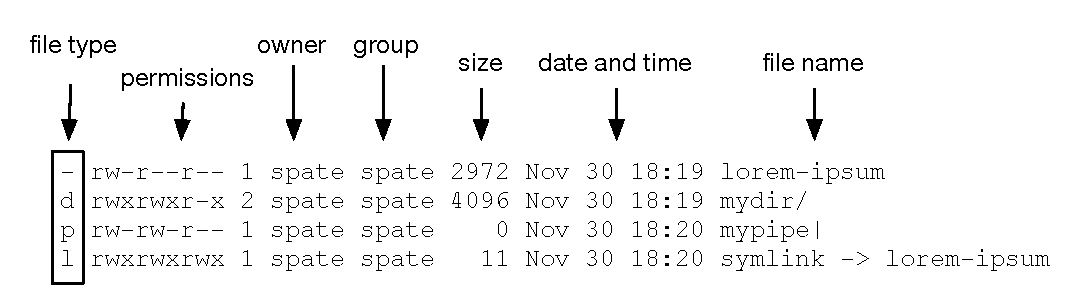
\includegraphics[scale=0.6]{figures/ls-l.pdf}
	\centering
	\caption{The Components of a File as Shown by Running \cf{ls -l}}
	\label{fig:ls-l}
\end{figure}

\section{File Descriptors}

Every time a file is opened or a file is created, a file descriptor is returned that can be used to reference the open file through uses of one of several different operations such as \cf{read(2)}, \cf{write(2)} and \cf{lseek(2)}. File descriptors are allocated on a per-process basis and are always non-negative. The first 3 file descriptors are reserved as shown in table \ref{table:fds}.

\begin{table}[h]
\begin{center}
\begin{tabular}{|p{0.1\textwidth}|m{0.1\textwidth}|m{0.3\textwidth}|m{0.3\textwidth}|}
\hline
\rowcolor[gray]{.93}\bf{Name}&\bf{Value}&\bf{<stdio.h> file stream}&\bf{\cf{<unistd.h>} constant}\\
\hline
\cf{stdin}&0&standard input&\cf{STDIN\_FILENO}\\
\hline
\cf{stdout}&1&standard output&\cf{STDOUT\_FILENO}\\
\hline
\cf{stderr}&2&standard error&\cf{STDERR\_FILENO}\\
\hline
\end{tabular}
\caption{\small Standard File Descriptors}
\label{table:fds}
\end{center}
\end{table}

\noindent
In the example below, you can see that the following program will receive the next available file descriptor which is 3.

\begin{lstlisting}
$ [*\bfseries cat fd.c*]
#include <stdio.h>
#include <fcntl.h>

int
main()
{
	int fd = open("lorem-ipsum", O_RDONLY);
	printf("fd = %d\n", fd);
}
$ [*\bfseries make fd*]
$ [*\bfseries ./fd*]
fd = 3
\end{lstlisting}

\noindent
Jumping ahead a little to demonstrate how file descriptors are used in the kernel, the \cf{read(2)} system call us handled by the kernel function \cf{ksys\_read()} of which I've included a fragment of the source code here:

\begin{lstlisting}
ssize_t [*\bfseries ksys\_read*](unsigned int fd, char __user *buf, 
                  size_t count)
{   
	struct fd f = [*\bfseries fdget\_pos*](fd);
	loff_t pos, *ppos = [*\bfseries file\_ppos*](f.file);
	ret = [*\bfseries vfs\_read*](f.file, buf, count, ppos);
\end{lstlisting}

\noindent
As you can see, the arguments are very similar to the \cf{read(2)} system call. Inside this function the kernel uses the file descriptor to get an \cf{fd} struct. From there, it gets the position from the last read (or seek) and calls \cf{vfs\_read()} to continue read processing. We'll explore the kernel side of reading later in section \cf{XXX}.

%------------------------------------------------------------------------------------------------------------------------------------------------------------

\subsection{How Many Open Files?}

Most applications only open a small number of files and the Linux kernel is set up to support this by default for each process. The \cf{getdtablesize(2)} manpage has conflicting information. It states that it returns the maximum number of files a process can have open. But then it lists the return value as the \textit{current limit}. The following program retrieves this value and also checks to see what is returned from calling \cf{getrlimit()} which returns both the current limit (also called the \textit{soft limit}) and the \textit{hard limit} as returned by calling \cf{getrlimit(2)}:

\begin{lstlisting}
#include <unistd.h>
#include <stdio.h>
#include <sys/resource.h>

int
main()
{
    struct rlimit  rlim;
    int            nentries;

    nentries = getdtablesize();
    getrlimit(RLIMIT_NOFILE, &rlim);
    printf("Current file table entries = %d\n", nentries);
    printf("rlimit current / maximum = %d / %d\n",
           (int)rlim.rlim_cur, (int)rlim.rlim_max);
}
\end{lstlisting}

\noindent
Here is what we get when running the program. 1,048,576 is certainly larger than most applications will need.

\begin{lstlisting}
Current file table entries = 1024
rlimit current / maximum = 1024 / 1048576
\end{lstlisting}

\noindent
You can also get the current limit by calling the shell built-in command "\cf{ulimit -Sn}" and calling "\cf{ulimit -Hn}" to get the hard limit.

%------------------------------------------------------------------------------------------------------------------------------------------------------------

\subsection{Closing Files}

There isn't a great deal to say about closing files. The system call, as described in \cf{close(2)} is as follows:

\begin{lstlisting}
#include <unistd.h>

int close(int fd);
\end{lstlisting}

\noindent
If there are any record locks held on the file that \cf{fd} refers to and are owned by the calling process, they are removed.

If \cf{fd} is the last file descriptor referring to the underlying open file any resources that associated with the open file are freed. If the file descriptor is the last reference to a file which has been removed by a prior call to \cf{unlink(2)}, the file will then be deleted. The latter point is an interesting one for filesystem developers as the file could remain in this state for an extended period of time and there are certainly implications if the system is restarted in between these two operations.

%------------------------------------------------------------------------------------------------------------------------------------------------------------

\subsection{Duplicating File Descriptors}

The \cf{dup(2)} system call can be called to allocate a new file descriptor which will reference the same open file as the descriptor \cf{oldfd}. The returned value is guaranteed to be the lowest-numbered file descriptor that is unused in the calling process.

\begin{lstlisting}
#include <unistd.h>

int dup(int oldfd);
int dup2(int oldfd, int newfd);
\end{lstlisting}

\noindent
Since both old and new file descriptors reference the same file, they can then be used interchangeably.  They also share file offset and file status flags. If the file offset is changed by using the \cf{lseek(2)} system call on one of the file descriptors, the offset will also changed for the other file descriptor.

The \cf{dup2(2)} system call is similar but instead of getting the lowest available file descriptor, the file descriptor specified by \cf{newfd} is used. If \cf{newfd} is currently in use, it is closed first. This function is the equivalent of calling \cf{fcntl(2)} and passing the \cf{F\_DUPFD} command.

The \cf{dup3(2)} system call was added to Linux version 2.6.27. It performs the same function as \cf{dup2(2)} with one exception. The caller can force the close-on-exec flag to be set  for  the  new file  descriptor by setting \cf{flags} to \cf{O\_CLOEXEC}.  In this case the file descriptor will be closed following a call to \cf{execve(2)}. The \cf{open(2)} manpage describes how this flag is useful in multithreaded applications.

\begin{lstlisting}
#include <fcntl.h> 
#include <unistd.h>

int dup3(int oldfd, int newfd, int flags);
\end{lstlisting}

\noindent
The most common use case for duplicating file descriptors is to connect processes via a pipe which is a common operation we all use when running one command in the shell and connecting the output to the input of the next command. In the following example:

\begin{lstlisting}
$ [*\bfseries find . -name *.c | xargs grep myfunc*]
\end{lstlisting}

\noindent
the output of the \cf{find} command is connected to the input of the \cf{xargs} command.

\subsubsection{An Example of Redirection}

This section is really going beyond the scope of this book but redirection is such a fundamental part of the UNIX/Linux shell, that I thought it was worth taking a slight diversion for readers who may not be familiar with how pipes are used to achieve one of UNIX's most fundamental and wonderful capabilities. 

Take a look at the following commands connected together where the standard output of \cf{echo} is connected to the standard input of \cf{cat}:

\begin{lstlisting}
$ [*\bfseries echo "Hello world" | cat*]
Hello world
\end{lstlisting}

\noindent
Below is a program that forks/execs two other programs (\cf{myecho} and \cf{mycat}) and uses a combination of \cf{dup(2)} and \cf{pipe(2)} to connect the two processes together through \cf{stdin} and \cf{stdout} in a simple but similar way to how the shell operates. When the \cf{shell} program is run we'll see our message displayed:

\begin{lstlisting}
$ [*\bfseries ./shell*]
Hello world!
\end{lstlisting}

\noindent
To see this visually, refer to figure \ref{fig:pipe}.

\begin{figure}
	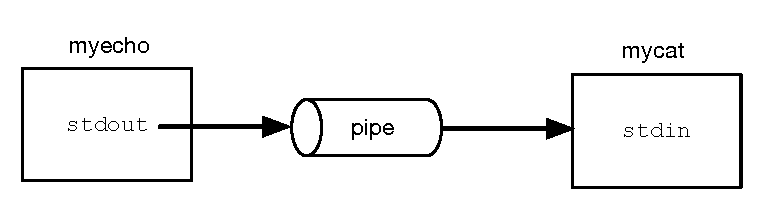
\includegraphics[scale=0.6]{figures/pipe.pdf}
	\centering
	\caption{Tow processes connected via a pipe}
	\label{fig:pipe}
\end{figure}

Below is the \cf{shell} program. As per usual, we've left out error checking for the purpose of keeping the number of lines as small as possible.

\begin{lstlisting}
 1 #include <unistd.h>
 2 #include <stdlib.h>
 3 #include <stdio.h>
 4 
 5 int main(int argc, char **argv) {
 6     int   pipefd[2];
 7     pid_t child;
 8 
 9     pipe(pipefd);
10     child = fork();
11  
12     if (child == 0) {
13         /* child process */
14         close(STDOUT_FILENO);
15         dup(pipefd[1]);
16         execlp("myecho", "myecho", "Hello world!\n",
17                (char *)NULL);
18     } else {
19         /* parent process */
20         close(STDIN_FILENO);
21         dup(pipefd[0]);
22         execlp("mycat", "mycat", (char *)NULL);
23     }
24 }
\end{lstlisting}

\noindent
The following bullet points describe what the various parts of the program are doing (line numbers are on the left):

\begin{itemize}
	\item line 9 -- A pipe is created where  \cf{pipe[0]} is the file descriptor through which we can read data
		and \cf{pipe[1]} is the file descriptor through which we can write data.
	\item line 10 -- The program is forked.
	\item line 14 -- \cf{stdout} is closed for the \cf{myecho} process.
	\item line 15 -- \cf{dup(2)} is called to duplicate the file descriptor in \cf{pipefd[1]} which is the \textit{write side}
		of the pipe. Recall that \cf{dup(2)} is guaranteed to return the lowest-numbered file descriptor that
		unused in the calling process. Since we have just closed \cf{stdout} which has a file descriptor of \cf{1},
		\cf{dup(2)} file descriptor 1 will be used which is \cf{stdout}.
	\item line 16 -- At this point we exec the \cf{myecho} program and pass \cf{"Hello world!"} as an argument.
	\item line 20 -- \cf{stdin} for the \cf{mycat} process is closed.
	\item line 21 -- Similar to line 15, we replace \cf{stdin} for \cf{mycat} with the \textit{read side} of the pipe.
	\item line 22 -- Finish with a call to exec the \cf{mycat} program.
\end{itemize}

\noindent
The actual shell is of course considerably more complicated than this program but in essence, this is what it is doing. 

Here is the \cf{myecho} program. It's very simple and just writes the argument passed to \cf{stdout}.

\begin{lstlisting}
#include <stdio.h>

int
main(int argc, char *argv[])
{
    fprintf(stdout, "%s", argv[1]);
}
\end{lstlisting}

\noindent
Here is the \cf{mycat} program. It reads from \cf{stdin} and writes the output (to \cf{stdout}.

\begin{lstlisting}
#include <stdio.h>
#include <string.h>

#define BUFSZ 64

int
main()
{
    char buf[BUFSZ];

    fgets(buf, BUFSZ, stdin);
    printf("%s", buf);
}
\end{lstlisting}

\noindent
Note that if you run these programs, make sure that \cf{PATH} is set to include the current directory so that the \cf{myecho} and \cf{mycat} programs can be found.

If you remove the comments around \cf{fprintf} you will see that for both processes, \cf{stderr} is still connected to the terminal on which the programs are run from:

\begin{lstlisting}
$ [*\bfseries ./shell*]
I'm mycat
I'm myecho
Hello world!
\end{lstlisting}

\subsection{Named Pipes}

A file type that can be supported by different filesystems is a named pipe.

\textbf{XXX---need to find out how Linux handles them}

There are some VFS interfaces/arguments for this. See section \ref{vfs-pipes} for the kernel side of things.

\section{Opening Files / Creating Files}

This section covers file creation together with the different file open operations since creation can also be performed using the \cf{open(2)} system call. The interfaces themselves are very simple but explanation is complicated by the large number of \textit{flags} that can be passed which determine how the file will be opened and accessed after open succeeds.

Here are the functions that can be used for open/create. They are described in the \cf{open2)} manpage with the exception of \cf{openat2(2)} which has its own manpage.

\begin{lstlisting}
#include <fcntl.h>

int open(const char *pathname, int flags);
int open(const char *pathname, int flags, mode_t mode);

int creat(const char *pathname, mode_t mode);

int openat(int dirfd, const char *pathname, int flags);
int openat(int dirfd, const char *pathname, int flags,
           mode_t mode);

int openat2(int dirfd, const char *pathname,
            const struct open_how *how, size_t size);
\end{lstlisting}

\noindent
In the first instance of open, \cf{pathname} references the file to be opened and can be relative or absolute, for example:

\vspace{10px}
    \cf{/home/spate/src/spfs/kern/sp\_dir.c} --- an absolute pathname
    
\vspace{5px}
     \cf{sp\_dir.c} --- a relative pathname
\vspace{10px}

\noindent
Absolute pathnames always start with '\cf{/}' and relative pathnames start from the current working directory which can be obtained with a call to \cf{getcwd(3)}.

The \cf{flags} argument must be one of \cf{O\_RDONLY},  \cf{O\_WRONLY},  or  \cf{O\_RDWR} for reading, writing or reading and writing. If a file is being created, \cf{O\_CREAT} should be OR'd with \cf{flags}.

There is a separate \cf{creat(2)} system call which is equivalent to calling \cf{open(2)} with \cf{flags} equal to \cf{O\_CREAT|O\_WRONLY|O\_TRUNC}.

\subsection{Open Flags}\label{prog-open-flags}

There are 19 different flags that can be passed to the \cf{open(2)} system call. This section will spent quite a but of time explaining each of the flags since the kernel has many conditional paths based on which flags are set. Note that are a few flags that are not related to file access and have been omitted from this list.

\begin{itemize}
	\item \cf{O\_APPEND} -- the file is opened in append mode so the file offset will be positioned at the end of the file.
	\item \cf{O\_CLOEXEC} -- enable  the close-on-exec flag for the new file descriptor otherwise the file descriptor will
		remain open in the child process following an \cf{execve(2)} system call.
	\item \cf{O\_CREAT} -- if the file does not exist, it is created as a regular file.
	\item \cf{O\_DIRECT} -- used by applications that wish to do their own caching (databases for example). I/O will move
		directly between the user address space buffers and disk.
	\item \cf{O\_DIRECTORY} -- if \cf{pathname} is not a directory, cause the open to fail. This
              flag was added to  avoid denial-of-service  problems.
	\item \cf{O\_DSYNC} -- if this flag is set, when a \cf{write(2)} system call (or similar calls) return, the data will have
              been transferred to the underlying hardware, along with any file metadata  that would be required to retrieve that data
              at a later date.
	\item \cf{O\_EXCL} -- this flag should be used in conjunction with \cf{O\_CREAT}. If the file already exists, the open 
		will fail. If the file does not exist, an attempt will be made to create it and open it. This allows a process to create 
		a file for writing and sure that no other process will write to. It could used for example, when creating a files in \cf{/tmp},
		where several other processes are creating files with similar, possibly identical, names. The \cf{mkstemp(3)} function 
		calls open with \cf{O\_CREAT} and \cf{O\_EXCL}.
	\item \cf{O\_LARGEFILE} -- allows files whose sizes cannot be represented in an \cf{off\_t}
              (but can be represented  in  an  \cf{off64\_t})  to  be  opened.   The \cf{\_LARGEFILE64\_SOURCE}  macro must 
              be defined (before including any header files) in order to obtain this definition.
	\item \cf{O\_NOATIME} -- do  not update the file's last access time (\cf{st\_atime} in the inode) when the file is read
		using \cf{read(2)} and friends.
	\item \cf{O\_NOFOLLOW} -- if the basename of \cf{pathname} is a symbolic link, the open will fail 
		with the error \cf{ELOOP}. 
	\item \cf{O\_NONBLOCK} -- when this flag is added, any operation including the open will not cause the calling process
		to wait. This flag is particularly useful when opening pipes. 
	\item \cf{O\_NDELAY} -- same as \cf{O\_NONBLOCK}.
	\item \cf{O\_PATH} -- this is an interesting flag. The goal is to obtain a file descriptor that can be used  to  indicate  a 
		\textit{location in the filesystem tree} and to perform operations that act  purely  at  the  file  descriptor level.  
		The file itself is not opened, and other file operations  (e.g.,  \cf{read(2)},  \cf{write(2)},  \cf{fchmod(2)},  \cf{fchown(2)}, 
		\cf{fgetxattr(2)}, \cf{ioctl(2)}, \cf{mmap(2)}) fail with the error \cf{EBADF}. Another use of this flag is in conjunction
		with the the "\cf{*at}" calls.
	\item \cf{O\_SYNC} -- this flag ensures that by the time a \cf{write(2)} (or similar) system call returns, the data and
              associated file metadata will have been transferred to the underlying hardware.
	\item \cf{O\_TMPFILE} -- create an unnamed temporary regular file.  The \cf{pathname} argument specifies a directory. 
		An unnamed inode will be created in the specified directory's filesystem.  Anything written to the resultin  file will be 
		lost when the last file descriptor is closed, unless the file is given a name.
	\item \cf{O\_TRUNC} -- if  the file already exists and it is a regular file and the access mode allows writing 
		(\cf{O\_RDWR} o  \cf{O\_WRONLY})  the file will be truncated to length 0.
\end{itemize}

\noindent
There is a lot of detail behind several of these flags. For example, I suggest exploring the use cases for \cf{O\_PATH}. As mentioned above, the kernel is littered with checks for these flags. Just taking \cf{O\_TMPFILE} as one example, here are the places in the kernel's \cf{fs} directory that reference this flag:

\begin{lstlisting}
$ [*\bfseries grep O\_TMPFILE *.c*]
namei.c:	if (unlikely(file->f_flags & __O_TMPFILE)) {
open.c:#define WILL_CREATE(flags) (flags & (__O_TMPFILE | ...
open.c:	 * O_TMPFILE on old kernels, O_TMPFILE is ...
open.c:	if (flags & __O_TMPFILE) {
open.c:		if ((flags & O_TMPFILE_MASK) != O_TMPFILE)
open.c:		if (flags & (O_TRUNC | O_CREAT | O_TMPFILE))
\end{lstlisting}

\noindent
Subsequent chapters will cover the kernel side of these flags.

%%%%%%%%%%%%%%%%%%%%%%%%%%%%%%%%%%%%%%%%%%%%%%%%%%%%%%%%%%%%

\section{Reading and Writing Files}

Reading from and writing to regular files was originally implemented by the \cf{read(2)} and \cf{write(2)} systems calls and enhanced by the standard I/O library which will be discussed in section \ref{stdio}. Over time there have been several other library and system call interfaces that support file I/O. To start, let's look at the original system calls:

\begin{lstlisting}
#include <unistd.h>

ssize_t read(int fd, void *buf, size_t count);
ssize_t write(int fd, const void *buf, size_t count);
\end{lstlisting}

\noindent
To read from a file, specify a valid file descriptor (\cf{fd}), a buffer in memory (\cf{buf}) and the number of bytes to be read. Reading will start from the current offset and the number of bytes read will be returned. Writing is the opposite. Starting from the current offset, an attempt will be made to write \cf{count} bytes from the address referenced by \cf{buf} to the file referenced by \cf{fd}.

When the file is opened, the offset is set to 0 and after each read or write operation, the offset will be advanced by the amount of data read or written.

Applications don't always wish to read and write sequentially so this is where the \cf{lseek(2)} system call comes into play:

\begin{lstlisting}
#include <unistd.h>

off_t lseek(int fd, off_t offset, int whence);
\end{lstlisting}

\noindent
The \cf{offset} argument specifies the offset within the file to move to and \cf{whence} can be one of the following:

\begin{itemize}
	\item \cf{SEEK\_SET} -- the file offset is set to \cf{offset} bytes.
	\item \cf{SEEK\_SET} -- the file offset is set to its current file location plus \cf{offset} bytes.
	\item \cf{SEEK\_SET} -- the file offset is set to the size of the file plus \cf{offset} bytes.
	\item \cf{SEEK\_DATA} -- the file offset is set to the next location in the file that is greater than or equal to the
		specified \cf{offset} containing data.
	\item \cf{SEEK\_HOLE} -- the file offset is set to the next hole in the file that is greater than or equal to \cf{offset}. 
		If \cf{offset} points into the middle of a hole, the file offset is set to \cf{offset}.  If there is no hole past
		offset, the file offset is adjusted to the end of the file.
\end{itemize}

\noindent
The last two options were added in Linux 3.1 to allow applications to handle holes in sparse files. One particular use case is file  backup tools, which can save space when creating backups by preserving holes. 

For applications that move around with a file frequently, both read/write and lseek calls can be combined together in a single call using one of the following two system calls:

\begin{lstlisting}
#include <unistd.h>

ssize_t pread(int fd, void *buf, size_t count, off_t offset);
ssize_t pwrite(int fd, const void *buf, size_t count, 
               off_t offset);
\end{lstlisting}

\noindent
Both functions differ from \cf{read(2)} and \cf{write(2)} in that although reads/writes occur from the specified offset, the current file offset is not changed. These two system calls are particularly useful for multi-threaded applications where different threads may be operating on the file at the same time. It would not be very useful for one thread to call \cf{lseek(2)} followed by \cf{write(2)} only to find that another thread had made a call to \cf{lseek(2)} in the meantime and changed the offset!

%%%%%%%%%%%%%%%%%%%%%%%%%%%%%%%%%%%%%%%%%%%%%%%%%%%%%%%%%%%%

\section{Vectored Reads and Writes}

There are times when applications know ahead of time that they will need to perform multiple I/Os to/from different memory addresses and the file, and likely at different offsets. This type of I/O is called \textit{vectored reads/writes} and also known as \textit{scatter/gather I/O}. There are several functions that can be used all of which utilize the \cf{iovec} structure, defined in \cf{<sys/uio.h>}:

\begin{lstlisting}
struct iovec {
    void  *iov_base;    /* Starting address */
    size_t iov_len;     /* Number of bytes to transfer */
};
\end{lstlisting}

\noindent
Figure \ref{fig:readv} highlights a case where we have four different I/Os that need to be performed. Each I/O is of a different length and the base address of the data inside the process's address space is at a different location. 

\begin{figure}
	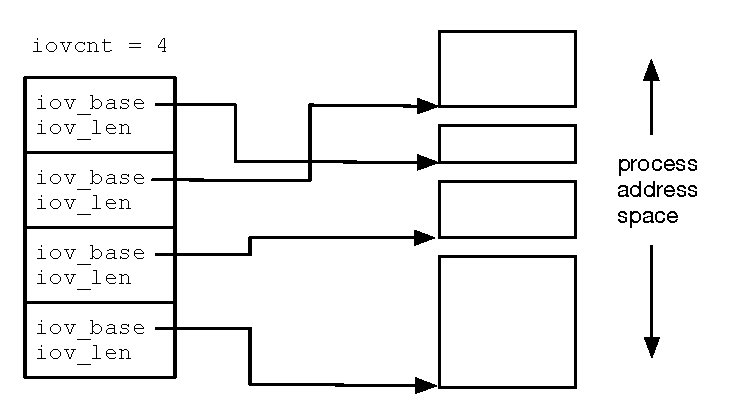
\includegraphics[scale=0.6]{figures/readv.pdf}
	\centering
	\caption{Issues multiple I/Os in a single system call using \cf{readv(2)} / \cf{writev(2)}}
	\label{fig:readv}
\end{figure}

Here are the functions that are available to perform vectored I/O. All are described by the \cf{readv(2)} manpage. The first two functions read / write from the current offset within the file. In figure \ref{fig:readv} there are four I/Os to different locations in memory but the data must be consecutive on disk.

\begin{lstlisting}
#include <sys/uio.h>

ssize_t readv(int fd, const struct iovec *iov, int iovcnt);
ssize_t writev(int fd, const struct iovec *iov, int iovcnt);

ssize_t preadv(int fd, const struct iovec *iov, int iovcnt,
               off_t offset);
ssize_t pwritev(int fd, const struct iovec *iov, int iovcnt,
                off_t offset);

ssize_t preadv2(int fd, const struct iovec *iov, int iovcnt,
                off_t offset, int flags);
ssize_t pwritev2(int fd, const struct iovec *iov, int iovcnt,
                 off_t offset, int flags);
\end{lstlisting}

\noindent
The \cf{preadv()} and \cf{pwritev()} functions combine reads/lseeks so that I/Os can take place from different offsets within the file as well as different areas in memory.

There are two main advantages of vectored I/O. The first is the reduction in the number of system calls that the application needs to make. Secondly if an application wishes to read data from a file into different locations in memory, using the \cf{read(2)} system call, the data would need to be read into a contiguous buffer in memory and then copied to the desired locations.

Here is an example of using both the \cf{readv()} and \cf{preadv()} functions in the same program. We start with a file of data that we're going to read which has ten \cf{0}s followed by ten \cf{1}s and so on:

\begin{lstlisting}
$ [*\bfseries cat vector-file*]
0000000000111111111122222222223333333333444444444455555555556666
666666777777777788888888889999999999
\end{lstlisting}

\noindent
The program source code is as follows:

\begin{lstlisting}
 1 #include <fcntl.h>
 2 #include <stdio.h>
 3 #include <unistd.h>
 4 #include <sys/uio.h>
 5  
 6 int
 7 main(int argc, char *argv[])
 8 {
 9     int  fd;
10     char buf2[32];
11     char buf3[32];
12     char buf1[32];
13     struct iovec bufs[] = {
14         { .iov_base = (void *)buf1, .iov_len = 10 },
15         { .iov_base = (void *)buf2, .iov_len = 10 },
16         { .iov_base = (void *)buf3, .iov_len = 10 },
17     };
18  
19     fd = open("vector-file", O_RDONLY);
20     lseek(fd, 10, SEEK_SET);
21     readv(fd, bufs, sizeof(bufs) / sizeof(bufs[0]));
22     printf("buf1 = %.10s\n", buf1);
23     printf("buf2 = %.10s\n", buf2);
24     printf("buf3 = %.10s\n", buf3);
25  
26     preadv(fd, bufs, sizeof(bufs) / sizeof(bufs[0]), 20);
27     printf("buf1 = %.10s\n", buf1);
28     printf("buf2 = %.10s\n", buf2);
29     printf("buf3 = %.10s\n", buf3);
30 }
\end{lstlisting}

\noindent
Here are the main points to discuss for this program:

\begin{itemize}
	\item line 10 - 12 -- we're allocating the buffers to read in to from the stack. But note that they'd been
		switched around so that they're not contiguous. Any order would work just the same.
	\item line 13 - 17 -- here are the definition of the \cf{iovec} structures to be used. There will be 3 reads of 10 bytes each.
	\item line 19 -- the file is opened read-only.
	\item line 20 -- a call is made to \cf{lseek(2)} to seek to byte 10 so the \cf{0}s will be skipped.
	\item line 21 -- the I/O call is issued.
	\item line 22 - 24 -- the first ten characters of each buffer is printed.
	\item line 26 -- this time the \cf{preadv(2)} system call is called. Prior to this call the file offset was changed to 40 following
		the call to \cf{readv(2)}. This time, we want to read starting at offset \cf{20}.
	\item line 27 - 29 -- print out ten characters from each buffer again.
\end{itemize}

\noindent
Here is the output when running the program:

\begin{lstlisting}
buf1 = 1111111111
buf2 = 2222222222
buf3 = 3333333333
buf1 = 2222222222
buf2 = 3333333333
buf3 = 4444444444
\end{lstlisting}

\noindent
Vectored I/O became popular with databases where large amount of I/O were needed but to different locations in memory where the database cached data. The basic interfaces were enhanced to allow different offsets in the file for each I/O. File I/O was later enhanced to avoid kernel caching (direct I/O) followed by backgrounding multiple I/Os, all to improve performance. Direct I/O and Async I/O will be described later in the chapter. 

%%%%%%%%%%%%%%%%%%%%%%%%%%%%%%%%%%%%%%%%%%%%%%%%%%%%%%%%%%%%%%%

\section{File and Record Locking}\label{prog-locking}

In a single application, a file can be accessed by multiple processes or by multiple threads within a single process. To handle synchronization between threads in a single processes there are various locking primitives that can be used by threads within the process. If multiple processes are accessing a file simultaneously, there are a different set of file and record locking interfaces that can be used to coordinate access. Historically, file locking has been a bit of a mess.

Some of these interfaces predate per-process multi-threading support. In particular, \textit{ddvisory} and \textit{mandatory} file locking have been around for many years and come with a set of issues that developers should be aware of. 

%------------------------------------------------------------------------------------------------------------------------------------------------------------

\subsection{Advisory File Locking}

The first type of file locking introduced in UNIX and available in Linux, was \textit{advisory locking} also called record locking since byte ranges within a file can be locked but processes must query to determine what portions of the file are locked. Thus the "advisory" part of the implementation.

To make things confusing, there are three functions that can be used for advisory locking namely \cf{fcntl(2)}, \cf{lockf(3)} and \cf{flock(2)}. On Linux, \cf{lockf(3)} is simply implemented on top of \cf{fcntl(2)} and any locks implemented through use of \cf{fnctl(2)} are ignored.

To get started, here is the interface for \cf{fcntl(2)}:

\begin{lstlisting}
#include <fcntl.h>

int fcntl(int fd, int cmd, ... /* arg */ );
\end{lstlisting}

\noindent
The \cf{cmd} argument will be \cf{F\_SET\_LK},  \cf{F\_SETLKW} or \cf{F\_GETLK} dependent on whether the caller wants to acquire, release or test for the existence of a record lock. The third argument passed is a pointer to an \cf{flock} structure which specifies what part of the file should be locked:
\begin{lstlisting}
struct flock {
   ... 
   short l_type;    /* Lock type: F_RDLCK, F_WRLCK, F_UNLCK */
   short l_whence;  /* How to interpret l_start. One of:
                           SEEK_SET, SEEK_CUR, SEEK_END */
   off_t l_start;   /* Starting offset for lock */
   off_t l_len;     /* Number of bytes to lock */
   pid_t l_pid;     /* PID of process blocking our lock
                       (set by F_GETLK and F_OFD_GETLK) */
   ... 
}; 
\end{lstlisting}

\noindent
The \cf{l\_type} field specifies whether the caller wants to take a read lock, a write lock or just unlock a previously locked set of bytes. The \cf{l\_whence},  \cf{l\_start} and \cf{l\_len} fields of this structure specify the range of bytes that the caller wishes to lock.

There is some deadlock detection built into the implementation such that if two processes attempt to access a region of the file that is locked by the other process, an \cf{EDEADLK} error will be returned and thus the caller should release some of its locks allowing others to proceed.

The implementation of this style of locking has other issues which will be described in section \ref{linux-adv-locking}.

%------------------------------------------------------------------------------------------------------------------------------------------------------------

\subsection{An Example of Advisory Locking}

This section shows two programs that work together to show how advisory locking can work between two processes. The first program (\cf{alock}) takes a write lock on the file "\cf{hello}" and over the whole file. It waits until it receives a signal (\cf{SIGUSR1} before releasing the lock.

The second program (\cf{lcat} calls the \cf{system(3)} library function to \cf{cat} the contents of the file. Before doing so, it checks three times to see if the file is locked. If it's still locked after the third check, it sends \cf{SIGUSR1} to the process that holds the lock. It can then display the file.

Here is the \cf{alock.c} program:

\begin{lstlisting}
 1 #include <unistd.h>
 2 #include <fcntl.h>
 3 #include <signal.h>
 4 #include <stdio.h>
 5 
 6 void
 7 mysig_hdlr(int signo)
 8 {
 9     printf("alock - got signal\n");
10     return;
11 }
12 
13 int
14 main()
15 {
16     struct flock     lock;
17     int              fd;
18     struct sigaction action;
19 
20     action.sa_handler = mysig_hdlr;
21     sigemptyset(&action.sa_mask);
22     action.sa_flags = 0;
23     sigaction(SIGUSR1, &action, NULL);
24 
25     fd = open("hello", O_RDWR);
26 
27     lock.l_type = F_WRLCK;
28     lock.l_whence = SEEK_SET;
29     lock.l_start = 0;
30     lock.l_len = 0;
31     lock.l_pid = getpid();
32     fcntl(fd, F_SETLK, &lock);
33     
34     printf("alock - file now locked\n");
35     pause();
36     lock.l_type = F_UNLCK;
37     fcntl(fd, F_SETLK, &lock);
38     printf("alock - file now unlocked\n");
39 }
\end{lstlisting}

\noindent
Some comments on the code:

\begin{itemize}
	\item lines 20 - 23 -- set up a signal handler (\cf{mysig\_hdlr}) for \cf{SIGUSR1}.
	\item lines 27 - 32 -- set a write lock on the file for the whole file by setting \cf{l\_start} to \cf{0} and \cf{l\_len} to \cf{0}. 
	\item line 35 -- pause waiting for \cf{SIGUSR1}.
	\item lines 36 - 37 -- release the lock (keeping the original fields that specify the start/length which is the whole file).
\end{itemize}

\noindent
Here is the source code for the \cf{lcat.c} program:

\begin{lstlisting}
 1 #include <signal.h>
 2 #include <stdlib.h>
 3 #include <unistd.h>
 4 #include <fcntl.h>
 5 #include <stdio.h>
 6 
 7 pid_t
 8 file_is_locked(int fd)
 9 {
10     struct flock    lock;
11 
12     lock.l_type = F_RDLCK;
13     lock.l_whence = SEEK_SET;
14     lock.l_start = 0;
15     lock.l_len = 0;
16     lock.l_pid = 0;
17 
18     fcntl(fd, F_GETLK, &lock);
19     return (lock.l_type == F_UNLCK) ? 0 : lock.l_pid;
20 }
21 
22 int main()
23 {
24     pid_t  pid;
25     int    i, fd;
26 
27     fd = open("hello", O_RDONLY);
28 
29     for (i = 0 ; i < 3 ; i++) {
30         if ((pid = file_is_locked(fd)) != 0) {
31             printf("lcat - waiting for lock\n");
32             sleep(1);
33         } else {
34             system("cat hello"); /* shouldn't get here */
35         }
36     }
37     printf("pid = %d\n", pid);
38     kill(pid, SIGUSR1);
39     sleep(1);
40     if ((pid = file_is_locked(fd)) == 0) {
41         system("cat hello");
42     } else {
43         /* shouldn't get here */
44         printf("lcat - lock still not released\n");
45     }
46 }
\end{lstlisting}

\noindent
Some comments on the code:

\begin{itemize}
	\item lines 10 - 19 -- the \cf{file\_is\_locked()} function checks to see if this process can take a read lock over
		the whole file. If it can it returns 0 and if it can't it returns the PID of the process that holds a lock that covers
		this range.
	\item lines 29 - 34 --  this program loops three times checking to see if the read lock can be taken. There is 
		nothing special about this loop. The idea is just that if the lock can't be taken, the program could be doing
		something else. After the 3rd attempt, it drops out with the PID of the process that holds the lock.
	\item line 38 - 39 -- send SIGUSR1 to the process that holds the lock. The \cf{alock} process will catch the signal
		and release the lock. It then waits a second to give \cf{alock} time to process the signal and unlock the file.
	\item lines 40 - 41 -- another check is made to see if \cf{lcat} can get the read lock. If it can, it will \cf{cat}
		the contents of the file.
\end{itemize}

\noindent
There are two places in the program where it states that the code path should not get there. This is certainly the case if only these two processes are accessing the file. If there are others, this could change. On line 43, this path could be reached if the "1" second sleep isn't enough to allow \cf{alock} to unlock the file.

Here are the two programs running in separate terminals but with the output merged so you can see the order of events:

\begin{lstlisting}
$ [*\bfseries ./alock*]                  |   
alock - file now locked    | 
                           | $ [*\bfseries ./lcat*]
                           | lcat - waiting for lock 
                           | lcat - waiting for lock 
                           | lcat - waiting for lock 
alock - got signal         | 
alock - file now unlocked  | 
                           | pid = 9671
                           | Hello world!
\end{lstlisting}

\noindent
Since this is advisory locking, applications must work in coordination with each other and non-cooperating applications cannit interfere otherwise assumptions will be broken. It would be best to segregate these applications and files so that no other users/processes can get access to them.

%------------------------------------------------------------------------------------------------------------------------------------------------------------

\subsection{Viewing Existing Locks}

Existing locks currently in use can be view in two ways. The first is to use the \cf{lslocks(1)} command:

\begin{lstlisting}
$ [*\bfseries lslocks -b*]
COMMAND     PID  TYPE  SIZE MODE  M START END PATH
multipathd  441  POSIX      WRITE 0     0   0 /run/snapd/ns...
cron        838  FLOCK      WRITE 0     0   0 /run/snapd/ns...
snapd       653  FLOCK      WRITE 0     0   0 /...
alock     10397  POSIX  13  WRITE 0     0   0 /home/.../hello
\end{lstlisting}

\noindent
In the last line you can see the \cf{alock} process that holds the \cf{WRITE} lock for \cf{13} bytes which is the length of the file. The type of lock depends on the call made. POSIX locks are created using the lockf(2) or \cf{fcntl(2)} system calls and FLOCK locks are created using the \cf{flock(2)} system call. 

The second method is to view the locks through \cf{/proc} as follows:

\begin{lstlisting}
$ [*\bfseries cat /proc/locks*]
1: POSIX  ADVISORY  WRITE 10397 fd:00:396261 0 EOF
2: FLOCK  ADVISORY  WRITE 653 fd:00:528747 0 EOF
3: FLOCK  ADVISORY  WRITE 838 00:1b:1248 0 EOF
4: POSIX  ADVISORY  WRITE 441 00:1b:506 0 EOF
$ [*\bfseries ps -ef | grep 10397*]
spate      10397    4862  0 23:35 pts/1    00:00:00 ./alock
\end{lstlisting}

\noindent
The obvious difference here is that there the command name is not shown although the process ID is displayed and can be easily used to find the process.

%------------------------------------------------------------------------------------------------------------------------------------------------------------

\subsection{Mandatory File Locking}

Since not all processes check for file locks, it was deemed that advisory locking needed a fix. The solution was the introduction of \textit{mandatory file locking} in SVR3 UNIX whereby access to a file would be denied if it was locked regardless of whether a process checks for locks or not. The intention of the scheme was to have as little impact as possible on existing applications. Of course, applications needed to be aware about how to handle the denial case. And to make matters worse, system calls such as \cf{unlink(2)} were able to succeed.

To enable mandatory file locking in Linux there are two steps that are needed:

\begin{enumerate}
	\item The underlying file system must be mounted with the \cf{mand} option (for example "\cf{mount -o mand -t 
		spfs /dev/sdb1 /mnt}").
	\item For the file to be locked, the set-group-ID bit must be turned on and the group-execute bit must be turned off for all
		files that need to be locked (for example "\cf{chmod g+s,g-x <file>}"). This is a combination that otherwise makes
		no sense. You can't get an uglier solution than this!
\end{enumerate}

\noindent
After a process places a mandatory lock on a file, no other process can access the file for reading or writing. 

As the \cf{Documentation/filesystems/mandatory-locking.txt} file in the kernel source tree indicates, there are several problems with mandatory locking. Firstly, "\textit{the write system call checks for a mandatory lock only once at its start.  It is therefore possible for a lock request to be granted after this check but before the data is modified. A process may then see file data change even while a mandatory lock was held."} There are also problems with \cf{read(2)} and \cf{mmap(2)}. Please consult this document if you have further interest in the issues surrounding mandatory file locking.

In Linux it's very clear that there is no love for mandatory locking and there have been attempts to remove it for many years. The "\textit{no regressions}" rule such that APIs cannot be removed in case it breaks an old application have resulted in the code still being there even though it's unknown whether anything still used mandatory locks.

As such, no further time will be given to mandatory locking.

%------------------------------------------------------------------------------------------------------------------------------------------------------------

\subsection{Open File Description Locks}\label{linux-adv-locking}

Linux introduced file-private POSIX locks in the 3.x kernel series with the goal of taking elements of both BSD-style and POSIX-style locks and combining them into a more robust locking API by removing some of the ambiguity that existed across the various UNIX platforms. The following article describes the work that was done and covers some of the problems that were solved. It also provides an example of using open file description locks in a multi-threaded environment. This section will highlight those changes.

\begin{table}[h]
\begin{tabular}{lcl}
\parbox[r]{0.5in}{
\includegraphics[scale=0.15]{figures/url.png}} & \parbox[l]{0.55in}{URL \arabic{urls}} & \parbox[l]{3in}{\cf{https://lwn.net/Articles/586904/}}
\end{tabular}
\end{table}
\stepcounter{urls}
% https://lwn.net/Articles/586904/

\noindent
One specific problem with POSIX locks is that when a request for a lock is made that would conflict with an existing lock previously taken by the same process, the kernel treats it as a request to modify the existing lock. This makes POSIX locks as good as useless in a multi-threaded application. 

If a process closes a file then all locks will be released even if a lock was taking using a different file descriptor (see \cf{dup(2)} and friends). Also, as the above article states "\textit{This is a particular problem for applications that use complex libraries that do file access. It's common to have a library routine that opens a file, reads or writes to it, and then closes it again, without the calling application ever being aware that has occurred. If the application happens to be holding a lock on the file when that occurs, it can lose that lock without ever being aware of it. That sort of behavior can lead to silent data corruption, and loss of developer sanity.}". This could be, and has been, a very difficult problem to debug.

In general, if you need to use advisory locking, use the newer Open File Description Locks and avoid using POSIX-style locking.

%%%%%%%%%%%%%%%%%%%%%%%%%%%%%%%%%%%%%%%%%%%%%%%%%%%%%%%%%%%%%%%

\section{Synchronizing I/O Operations}

Generally speaking, when data is written to a file, it is not automatically written to disk but written to the page cache that resides in the Linux kernel address space. Modified data will eventually be written to disk. Obviously this presents an issue if the system were to crash prior to this data being written. The same is true of the file's metadata which could include the file size.

There are two system calls that allow for flushing modified data and metadata that may be sitting in kernel caches that have not yet made it to disk. Both are described in the \cf{fsync(2)} manpage:

\begin{lstlisting}
#include <unistd.h>

int fsync(int fd);
int fdatasync(int fd);
\end{lstlisting}

\noindent
The \cf{fsync(2)} system call will flush any modified data that is still in memory. This includes any file data as well as file metadata (file attributes). This ensures that the changes will make it to disk such that if the system crashes, any data can still be retrieved.

The  \cf{fdatasync(2)} system call is similar but does not flush metadata. 

%%%%%%%%%%%%%%%%%%%%%%%%%%%%%%%%%%%%%%%%%%%%%%%%%%%%%%%%%%%%%%%

\section{Direct I/O}

% https://www.scylladb.com/2017/10/05/io-access-methods-scylla/ - good article

When file I/O occurs, data is cached in the kernel inside the \textit{page cache}. If data read or written is in the page cache it can be accessed without additional I/Os. This type of I/O is also called \textit{buffered I/O} since the data is \textit{buffered} in the kernel. Traditionally it was cached in the \textit{buffer cache}. 

Not all applications want data to be cached since they can better manage that cache themselves. The typical example is that of databases which allocate very large caches in the user address space.

Figure \ref{fig:direct-io} shows the three different paths that I/O can take. There are subtle differences between buffered I/O and mapped I/O.

\begin{figure}
	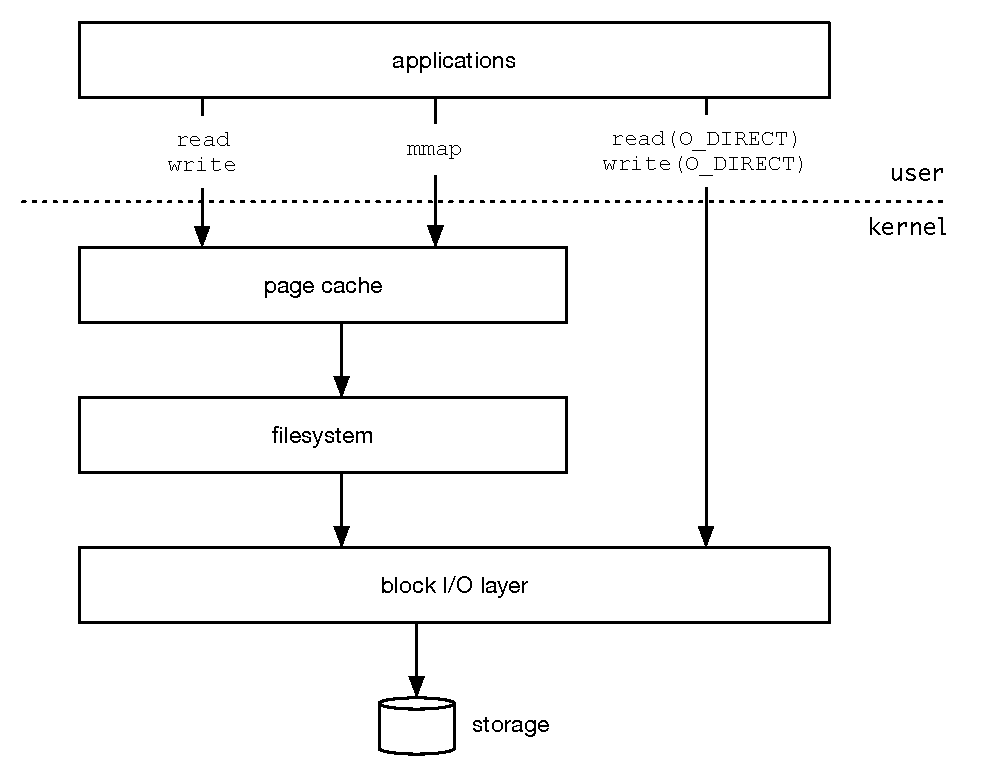
\includegraphics[scale=0.6]{figures/direct-io.pdf}
	\centering
	\caption{There are 3 paths to disk from applications}
	\label{fig:direct-io}
\end{figure}

\begin{enumerate}
	\item \textbf{Buffered I/O} -- this is the default type of I/O. Access goes through the filesystem and data is cached in
		the page cache. Strictly speaking, for writes, the data is written into page cache pages and at a later data, a call
		is made into the filesystem to flush them to disk. For reads, pages are allocated and a call is made into the 
		filesystem to read data from disk.
	\item \textbf{Memory mapping} -- applications access files through mappings into their address space. When data needs
		to be read or written, the kernel calls into the filesystem to perform the I/O. Once a page is in memory it will
		continue to be accessed through the mapping until a later date when data is flushed or the mapping is destroyed.
	\item \textbf{Direct I/O} -- the page cache is bypassed and data transfers directly between the process address space
		and disk.
\end{enumerate}

\noindent
Applications can request direct I/O by passing the \cf{O\_DIRECT} flag to the \cf{open(2)} system call. To enable direct I/O applications must be compiled with \cf{\_ALL\_SOURCE} enabled to see the definition of \cf{O\_DIRECT}.

The performance gains due to direct I/O are very dependent on the application's ability to effectively manage its own cache of data. There may be additional complexities if a file is being accessed through a mix of buffered I/O and direct I/O, certainly a situation that should be avoided.

Once a file is opened, reads and writes proceed as normal with the exception of alignment of user addresses and the amount of I/O requested. These restrictions are per-filesystem and there is no generic way in which to determine what the constraints imposed are.

\begin{itemize}
	\item The number of bytes to be transferred is a multiple of 512 bytes.
	\item The file offset is a multiple of 512 bytes.
	\item The user-supplied memory address is aligned on a 512-byte boundary.
\end{itemize}

\noindent
Note that some filesystems may have different requirements. For example, VxFS only requires a 8-byte boundary for the user address. XFS has the \cf{XFS\_IOC\_DIOINFO} command that can be passed to \cf{xfsctl(3)} to determine requirements.

There is no easy way to show direct I/O in progress or when it works or doesn't work. However, section \ref{kernel-direct-io} will describe the implementation of direct I/O and gives examples to show that the page cache is in fact bypassed.

%%%%%%%%%%%%%%%%%%%%%%%%%%%%%%%%%%%%%%%%%%%%%%%%%%%%%%%%%%%%

\section{Sparse Files}

A sparse file is a regular file that has one or more \textit{holes}. If you're not familiar with sparse files, that's going to sound like a very strange statement. Another way to put it is that a sparse file is a file that allows for efficient storage allocation for large amounts of data. If you've used virtual machines at any point in time, they're underpinned by sparse files. For example, consider a VM that has a 60 GB disk. When the VM is created, it doesn't need this much space and likely to be a small fraction. So why allocated 60 GB of disk space if it's not needed? This becomes a bigger problem as more and more VMs are created on the same storage infrastructure.

Sparse files are also useful when large parts of the file contain zeros. This avoids all data blocks being allocated up front. When data is written over a hole, new blocks will be allocated.

Sparse files can be found using the \cf{find(1)} command. For example, looking inside \cf{/var/log}, there are two sparse files:

\begin{lstlisting}
$ [*\bfseries sudo find /var/log -type f -printf "\%S\textbackslash t\%p\textbackslash n" | \textbackslash*]
  [*\bfseries gawk '\$1 < 1.0 {print}'*]
0.013824	/var/log/lastlog
0.127872	/var/log/faillog
\end{lstlisting}

\noindent
Selecting one of these files, \cf{ls(1)} can be used to view the file size and the number of blocks backing the file:

\begin{lstlisting}
$ [*\bfseries ls -lh /var/log/lastlog*]
-rw-rw-r-- 1 root utmp 290K Aug  1 17:16 /var/log/lastlog
$ [*\bfseries du -sh /var/log/lastlog*]
4.0K	/var/log/lastlog
\end{lstlisting}

\noindent
There is only 4 KB allocated to the file but the file size is 290 KB.

%------------------------------------------------------------------------------------------------------------------------------------------------------------------

\subsection{Sparse Files in Action}

Let's demonstrating with a small program which opens/creates a file, writes "\cf{hello}" at offset 0 then seeks to an offset of 16 KB and writes "\cf{world}". We're going to have to explore some details inside the filesystem to explain what's happening.

\begin{lstlisting}
#include <stdio.h>
#include <string.h>
#include <errno.h>
#include <unistd.h>
#include <fcntl.h>

char *buf1 = "hello";
char *buf2 = "world";

int
main(int argc, char *argv[])
{
    int fd = open("/mnt/foo", O_CREAT|O_WRONLY, 0700);
    write(fd, buf1, strlen(buf1));
    lseek(fd, 16384, SEEK_SET);
    write(fd, buf2, strlen(buf2));
}
\end{lstlisting}

\noindent
Now let's look at the file:

\begin{lstlisting}
# [*\bfseries ls -l /mnt/foo*]
-rwx------ 1 root root 16389 Dec 15 20:54 /mnt/foo
\end{lstlisting}

\noindent
This is the expected size of the file but what's after "\cf{hello}" and before we get to "\cf{world}" at an offset of 16384? The answer isn't always consistent and depends on the underlying filesystem and its properties. But to give one example and where a file is sparse, we've created this file on top of SPFS, the disk-based filesystem whose implementation will be described in chapter \ref{disk-fs}.

This particular filesystem has a block size of 2048 bytes. This is the minimum amount of space that can be allocated to any file. Ignoring our sparse file example, if we were to start writing sequentially to a file at 0, SPFS would allocate blocks to the file as follows:

\begin{itemize}
	\item bytes 0 - 2047 --- allocate block
	\item bytes 2048 - 4195 --- allocate block
	\item bytes 4196 - 6143 --- allocate block
	\item and so on
\end{itemize}

\noindent
If we only wrote 1 byte at offset 0, we'd get 1 block allocated. If we wrote 2048 bytes at offset 0 (for a total of 2049 bytes), we'd get two blocks allocated and so on.

Let's take a look at the file using the \cf{stat(1)} command:

\begin{lstlisting}
# [*\bfseries stat /mnt/foo*]
  File: /mnt/foo
  Size: 16389     	  [*\bfseries Blocks: 2*] IO Block: 2048 regular file
Device: 800h/2048d	  Inode: 4  Links: 1
Access: (0700/-rwx------) Uid: ( 0/  root)   Gid: ( 0/  root)
Access: 2022-12-15 20:54:09.000000000 +0000
Modify: 2022-12-15 20:54:09.000000000 +0000
Change: 2022-12-15 20:54:09.000000000 +0000
\end{lstlisting}

\noindent
There are 2 blocks allocated to this file as highlighted. Each block is 2048 bytes so that's a total of 4096 bytes. But our file is now 16389 bytes according to \cf{ls(1)}. Both are correct. The file is sparse so has a hole in the middle. Next, we are going to use the SPFS filesystem debugger and display the contents of the inode for the file that we've written. We'll cover inodes in detail later but just think of it as a filesystem structure that records information about a file. You can see the file size and also see that a block (131) has been allocated for block offset 0 and another block (132) has been allocated at block offset 8. There are no allocated blocks for block offsets 1 through 7.

\begin{lstlisting}
spfsdb > [*\bfseries i4*]
inode number 4
  i_mode     = 81c0
  i_nlink    = 1
  i_atime    = Thu Dec 15 20:54:09 2022
  i_mtime    = Thu Dec 15 20:54:09 2022
  i_ctime    = Thu Dec 15 20:54:09 2022
  i_uid      = 0
  i_gid      = 0
  i_size     = 16389
  [*\bfseries i\_blocks   = 2*]
  [*\bfseries i\_addr[ 0] = 131   i\_addr[ 8] = 132*]
\end{lstlisting}

\noindent
The layout of the file is shown pictorially in figure \ref{fig:sparse}. If the application were to read the file, it would see "\cf{hello}" followed by a lot of zeroes followed by "\cf{world}".

\begin{figure}
	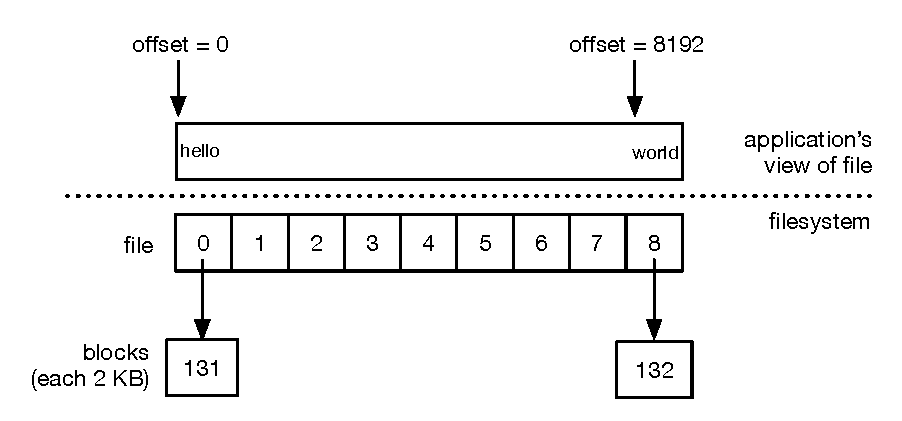
\includegraphics[scale=0.6]{figures/sparse.pdf}
	\centering
	\caption{A sparse file only showing 2 allocated blocks}
	\label{fig:sparse}
\end{figure}

In fact, this doesn't work - \textbf{XXX---bug - see notes. Needs fixing}

\subsection{Sparse File Example 1 --- Virtual Machines}

Virtual Machines are a wonderful application of how sparse files achieve the goal of mimicking large devices but only allocate data as and when needed. Disks are generally represented as sparse files in some underlying filesystem that is storing the virtual disks. When you create a virtual disk, under the covers, the hypervisor creates a sparse file on disk in a similar way to our simple program above. As the VM operating system writes blocks to disk, the hypervisor translates these writes into lseek/write combinations. Over time, you end up with a sparse file that has many holes and an ever increasing amount of allocated storage as the VM writes more and more data

In commercial implementations with 100s or 1000s of VMs, the cost savings can be huge. Storage does not need to all be allocated up front and can be added later as VM disks start to grow. Furthermore, data deduplication is typically deployed. 100s of VMs have a very similar footprint in terms of operating system binaries and such like.

%------------------------------------------------------------------------------------------------------------------------------------------------------------------

\subsection{Sparse File Example 2 --- HSM Applications}

An older but very relevant example of how sparse files were used by applications was for HSM (Hierarchal Storage Management) applications. There was a whole standard developed around this called DMIG (Data Management Interfaces Group). When I was at SCO, I used to travel from the UK to the US every 6 weeks or so to attend meetings. I got to visit several new cities and meet a lot of prominent operating system and filesystem engineers from the top companies at the time.

In the early 90s, disks were much smaller than you see today and also very expensive. Therefore to save space, several vendors developed what were then called HSM applications. The goal of such applications was to run periodically and perform the following:

\begin{itemize}
	\item Look for files that have not recently been accessed.
	\item Migrate the \textit{punched data} off to tape or other cheap storage.
	\item Punch a hole in the file. More likely, the hole would be from a specific offset to the end of the file.
	\item Make sure that the timestamps were not modified.
\end{itemize}

\noindent
A small amount of data was left at the start of each \textit{managed file} to satisfy requested from commands such as \cf{file(1)} which would read from the start of the file to determine file type. If a request was made to read/write to a portion of the file that had been migrated, the application would be paused while the data was read from tape and written back to the file.

Sound complicated? Yes it was and was made even more complicated by the fact that there was a lot of hacking of existing filesystems and parts of the kernel to make this work across different operating systems. And with several commercial versions of UNIX at the time, porting HSM applications was prohibitive. 

But this was a big enough problem and there was enough customer demand that the DMIG standard was developed and published and many operating system and filesystem vendors implemented support. Move forward twenty years and there is little information on the web now. In fact a Google search while writing this showed a fragment from my previous book on UNIX Filesystems but little else.

%%%%%%%%%%%%%%%%%%%%%%%%%%%%%%%%%%%%%%%%%%%%%%%%%%%%%%%%%%%%%%%

\section{Buffered I/O and the Standard I/O Library}\label{stdio}

We covered the \cf{read(2)} and \cf{write(2)} system calls earlier and other sections in this chapter cover specialized I/O capabilities such as vectored reads/writes and asynchronous I/O. This section describes how the standard I/O library operates.

As the \cf{stdio(3)} man page says:

\begin{quote}
\textit{The  standard  I/O  library  provides  a  simple and efficient buffered stream I/O interface.  Input and output is  mapped  into  logical  data streams  and the physical I/O characteristics are concealed.}
\end{quote}

\noindent
Figure \ref{fig:stdio-1} shows the position of the standard I/O library in relation to an application and the Linux kernel. Developers have two choices when operating on a file. They can use system calls directly or they can use the standard I/O library which contains a wide array of functions for dealing with file I/O. The \cf{stdio(3)} manpage provides a good overview of the standard I/O library and the functions that it provides. There are approximately 56 different functions available. All C developers will be familiar with the \cf{printf(3)} function including their first "\textit{Hello world}" program. Well, \cf{printf(3)} is one of the 56 functions and by default, it writes to the standard output file stream.

\begin{figure}
	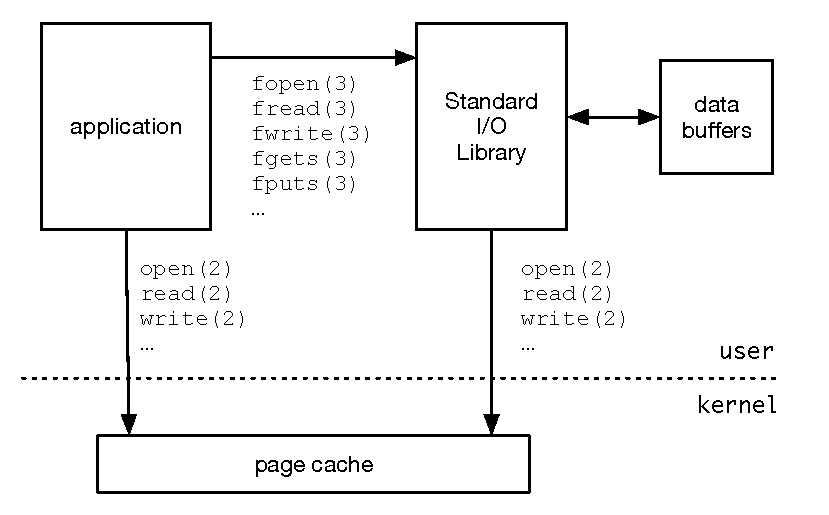
\includegraphics[scale=0.6]{figures/stdio-1.pdf}
	\centering
	\caption{Using the Standard Library vs System Calls}
	\label{fig:stdio-1}
\end{figure}

Whether to use system calls directly or use the standard library is very dependent on what your application does. If you are developing an application that processes text files, the standard library is generally the better choice. You can read/write single characters at a time, read lines terminated by newlines or format the data then write to a file stream. For the standard I/O library, \cf{printf(3)} and friends ease the job of formatting text to be written. The same is true for \cf{scanf(3)} and similar functions. If you use the system calls \cf{read(2)} and \cf{write(2)} and want to process text, you'll likely repeat the work that the standard I/O library has already done for you.

%------------------------------------------------------------------------------------------------------------------------------------------------------------------

\subsection{The Standard I/O Library \cf{FILE} Structure}

Let's take a look at a few functions provided by the standard I/O library. In all cases the \cf{stdio.h} header file needs to be included.

\begin{lstlisting}
#include <stdio.h>

FILE *[*\bfseries fopen*](const char * restrict path,
            const char * restrict mode);
int [*\bfseries fclose*](FILE *stream);
size_t [*\bfseries fread*](void *restrict ptr, size_t size,
             size_t nitems, FILE *restrict stream);
int [*\bfseries fscanf*](FILE *restrict stream, 
           const char *restrict format, ...);
\end{lstlisting}

\noindent
The standard library operates on a \textit{file stream} as defined by the \cf{FILE} structure. The \cf{stdio.h} header file doesn't contain the definition of \cf{struct FILE}. For that you need to look at the following header file:

\begin{lstlisting}
/usr/include/aarch64-linux-gnu/bits/types/FILE.h
typedef struct _IO_FILE FILE;
\end{lstlisting}

\noindent
which is part of the glibc source repository. To get to "\cf{struct \_IO\_FILE}" you need to look in the glibc sources:

\begin{itemize}
	\item In the glibc source code
	\subitem \cf{glibc/libio/bits/types/struct\_FILE.h}
    	\item On my Ubuntu VM under \cf{/usr/include}
	\subitem \cf{aarch64-linux-gnu/bits/types/struct\_FILE.h}  
\end{itemize}

\noindent
Here is part of the structure, specifically those fields that we'll be covering in this section to help understand how buffered I/O works:

\begin{lstlisting}
struct _IO_FILE
{
  int                _flags;     
  char              *_IO_read_ptr;
  char              *_IO_read_end;  
  char              *_IO_read_base;  
  char              *_IO_write_base; 
  char              *_IO_write_ptr; 
  char              *_IO_write_end;  
  char              *_IO_buf_base;
  char              *_IO_buf_end;  
  char              *_IO_save_base;
  char              *_IO_backup_base;  
  char              *_IO_save_end; 
  struct _IO_marker *_markers;
  struct _IO_FILE   *_chain;
  int                _fileno;
  int                _flags2;
  unsigned short     _cur_column;
  signed char        _vtable_offset;
  char               _shortbuf[1];
  _IO_lock_t        *_lock;
};
\end{lstlisting}

\noindent
One of the best ways to view what is happening when you use the standard I/O library is run a simple program under \cf{gdb}, set breakpoints and view the different fields in the \cf{FILE} structure. Here is a very simple program which will be used to demonstrate this point:

\begin{lstlisting}
 1  #include <stdio.h>
 2
 3  int
 4  main()
 5  {  
 6      FILE *fp;
 7      int         c; 
 8
 9      fp = fopen("lorem-ipsum", "r");
10      c = fgetc(fp);
11      printf("char = %c\n", (char)c);
12  }  
\end{lstlisting}

\noindent
The "\cf{lorem-ipsum}" file contains the commonly seen Latin text starting "\cf{Lorem ipsum dolor sit ...}" which is used throughout the book. In case you've ever wondered where this text came from, Wikipedia informs us that:

\begin{quote}
\textit{Lorem ipsum is typically a corrupted version of De finibus bonorum et malorum, a 1st-century BC text by the Roman statesman and philosopher Cicero, with words altered, added, and removed to make it nonsensical and improper Latin.}
\end{quote}

\noindent
In our \cf{gdb} session, we'll set a breakpoint, run the program and display the character read ("\cf{L}" as expected) as well as the contents of the \cf{FILE} structure:

\begin{lstlisting}
(gdb) [*\bfseries b 11*]
Breakpoint 1 at 0x840: file fget.c, line 11.
(gdb) [*\bfseries run*]
Starting program: /home/spate/spfs/test/fget 
[Thread debugging using libthread_db enabled]
Using host libthread_db library "/lib/aarch64-linux-gnu...
	
Breakpoint 1, main () at fget.c:11
11		printf("char = [*\%c\textbackslash*]n", (char)c);
(gdb) [*\bfseries p c*]
$1 = 76
(gdb) [*\bfseries p (char)c*]
$2 = 76 'L'
(gdb) [*\bfseries p *fp*]
$3 = {_flags = -72539000, 
  _IO_read_ptr = 0xaaaaaaac1481 "orem ipsum dolor sit amet"..., 
  _IO_read_end = 0xaaaaaaac201c "", 
  _IO_read_base = 0xaaaaaaac1480 "Lorem ipsum dolor sit"..., 
  _IO_write_ptr = 0xaaaaaaac1480 "Lorem ipsum dolor sit"..., 
  _IO_buf_base = 0xaaaaaaac1480 "Lorem ipsum dolor sit"..., 
  _IO_buf_end = 0xaaaaaaac2480 "", _IO_save_base = 0x0, 
  _IO_backup_base = 0x0, _IO_save_end = 0x0, _markers = 0x0, 
  _chain = 0xfffff7fa1520 <_IO_2_1_stderr_>, _fileno = 3, 
  _flags2 = 0, _old_offset = 0, _cur_column = 0, 
  _vtable_offset = 0 '\\000', _shortbuf = "",  
  _lock = 0xaaaaaaac1380, _offset = -1, _codecvt = 0x0, 
  _wide_data = 0xaaaaaaac1390, _freeres_list = 0x0, 
  _freeres_buf = 0x0,  __pad5 = 0, _mode = -1, 
  _unused2 = '\000' <repeats 19 times>}
\end{lstlisting}

\noindent
The \cf{\_fileno} field is the file descriptor referencing the open file. Since this is the only file used by the application other than the standard file descriptors, when the file is opened a file descriptor of 3 is returned.

The \cf{\_IO\_buf\_base} points to a a buffer in which data is read into and written from. The \cf{\_IO\_buf\_end} points to the end of the buffer so, in theory we have 4 KB of data that's been read from the file. But since the file is only 2,972 bytes in size we see that \cf{\_IO\_read\_end} is set to \cf{0x201c}. Subtracting the two we have \cf{0x201c – 0x1481 = 0xB9B} which in decimal is \cf{2971}. Since the first character of the file is stored at \cf{0x201c}, this makes \cf{2972}, the size of the file.

The \cf{\_IO\_read\_ptr} and \cf{\_IO\_write\_ptr} fields reference the position within this 4 KB buffer where we are currently reading and writing from/to. Since we've read a single character from the file, \cf{\_IO\_read\_ptr} is incremented to point to the next position in the buffer (the character "\cf{o}").

%------------------------------------------------------------------------------------------------------------------------------------------------------------------

\subsection{Analyzing the glibc Standard I/O Library}

You can download the most recent glibc source code as follows:

\begin{lstlisting}
# [*\bfseries git clone https://sourceware.org/git/glibc.git*]
# [*\bfseries cd glibc*]
# [*\bfseries git checkout master*]
\end{lstlisting}

\noindent
As an example of how to see what glibc is doing, navigate to the \cf{libio} directory and choose the field of the \cf{FILE} that you wish to analyze, for example:

\begin{lstlisting}
   # [*\bfseries grep \_IO\_read\_ptr *c*]
\end{lstlisting}

\noindent
You will see lots of references. To understand the flow through the library calls you'll need to spend some time analyzing the code. There are several indirections. For example, for \cf{fread(3)} start at \cf{\_IO\_fread()} in \cf{iofread.c} and go from there. You can also use the Elixir Cross Referencer, for example:

\begin{lstlisting}
https://elixir.bootlin.com/glibc/latest/source/libio/iofread.c
\end{lstlisting}

\noindent
I actually found it easier to grep. For example, search for the following:

\begin{lstlisting}
'fp->_IO_read_ptr'
'fp->_IO_read_ptr ='
[*\bfseries 'fp->\_IO\_read\_ptr+'*]
'fp->_IO_read_ptr-'
\end{lstlisting}

\noindent
and you'll see a smaller set of hits. For the highlighted option, there were only 3 hits:

\begin{lstlisting}
$ [*\bfseries grep 'fp->\_IO\_read\_ptr+' *c*]
genops.c:    return *(unsigned char *) fp->_IO_read_ptr++;
genops.c:	return *(unsigned char *) fp->_IO_read_ptr++;
genops.c:  return *(unsigned char *) fp->_IO_read_ptr++;
\end{lstlisting}

\noindent
Looking inside \cf{genops.c} in the function \cf{\_\_uflow()}, there is a fragment of code:

\begin{lstlisting}
if (fp->_IO_read_ptr < fp->_IO_read_end)
  return *(unsigned char *) fp->_IO_read_ptr++;
\end{lstlisting}

\noindent
A character is being returned from the current read pointer and the read pointer is being incremented as long as the read pointer still references data in the buffer (first line).

I started to experiment further by extending the program to do the following and printing out various pointers in the \cf{FILE} struct to see how the pointers changed. I was particularly curious when mixing reads and writes:

\begin{lstlisting}
c = fgetc(fp);
c = fgetc(fp);
c = fgetc(fp);
c = fputc('1', fp);
c = fputc('2', fp);
c = fputc('3', fp);
c = fgetc(fp);
\end{lstlisting}

\noindent
The result was not what I expected. After the first \cf{fgetc()}, I display two addresses and for each get/put call, I printed out \cf{\_IO\_read\_ptr} and \cf{\_IO\_write\_ptr} as follows:

\begin{lstlisting}
$ [*\bfseries ls -l lorem-ipsum*]
-rw-r--r-- 1 spate spate [*\bfseries 2972*] Dec 12 21:00 lorem-ipsum
$ [*\bfseries ./fget *]
_IO_read_base = 0xaaab0b8b3480
_IO_read_end  = 0xaaab0b8b401c ([*\bfseries 2972*] difference)

_IO_read_ptr    _IO_write_ptr
------------------------------
0xaaab0b8b3481  0xaaab0b8b3480
0xaaab0b8b3482  0xaaab0b8b3480
0xaaab0b8b3483  0xaaab0b8b3480
[*\bfseries 0xaaab0b8b401c*]  0xaaab0b8b3484
0xaaab0b8b401c  0xaaab0b8b3485
0xaaab0b8b401c  0xaaab0b8b3486
[*\bfseries 0xaaab0b8b3481*]  0xaaab0b8b3480
Character read = i
$ [*\bfseries head -1 lorem-ipsum*]
Lor123ipsum dolor sit amet, consectetur adipiscing
\end{lstlisting}

\noindent
This doesn't quite meet expectations. We know from the previous example that we get 'L', 'o' and 'r' for our first 3 \cf{fgetc()} calls and the read pointer advances through the buffer as expected. When we issue the first \cf{fputc()} call, we don't write at \cf{\_IO\_write\_ptr} but at \cf{\_IO\_read\_ptr}. This makes sense as we are advancing through the file. But after the first \cf{fputc()}, the value of \cf{\_IO\_read\_ptr} is set to \cf{\_IO\_read\_end}. Quite strange. And when we issue our final call to \cf{fgetc()} we get the character 'i' which is contained at offset \cf{\_IO\_write\_ptr}!

I decided at this point that finding the answer was really beyond the scope of this book since the goal was to introduce the standard I/O library, not to explain the details of how it works internally. But I was intrigued enough that I set it as a goal to write a future blog entry so please take a look at my website.

%%%%%%%%%%%%%%%%%%%%%%%%%%%%%%%%%%%%%%%%%%%%%%%%%%%%%%%%%%%%%%%

\section{Memory Mapped Files}\label{prog-mmap}

Memory mapped files were first introduced by Sun in their SunOS version 4 operating system in late 1988 (soon to be renamed Solaris) and described in the classic Usenix paper "\textit{Virtual Memory Architecture in SunOS}". I recommend reading it to find out the history of how UNIX moved from the buffer cache for all file I/O to a hybrid buffer cache / page cache. The new architecture allowed for the integration of all I/O to use the new virtual memory subsystem and a move away from the kernel buffer cache for file data. This architecture was adopted in the System V Release 4 version of UNIX and the architectural principles were later adopted in Linux.

\begin{table}[h]
\begin{tabular}{lcl}
\parbox[r]{0.5in}{ 
\includegraphics[scale=0.15]{figures/url.png}} & \parbox[l]{0.1in}{\arabic{urls}} & \parbox[l]{3in}{\cf{https://tinyurl.com/2p9cymm2}}
\end{tabular}
\end{table}
\stepcounter{urls}
% ttp://kos.enix.org/pub/gingell8.pdf

\noindent
The new architecture touched a large part of the operating system and soon after it was introduced, the development system was largely rewritten such that dynamic libraries made extensive use of \cf{mmap(2)}.

How does \cf{mmap(2)} work? Let's start with a simple example which opens a file and maps the whole file into memory. The call to \cf{mmap(2)} returns the user-space address to where the file is mapped. The program then proceeds through the mapping, one address at a time, writing each character read to \cf{stdout}.

\begin{lstlisting}
#include <sys/mman.h>
#include <sys/stat.h>
#include <fcntl.h>
#include <stdio.h>
#include <unistd.h>

int
main()
{
    struct stat st;
    char        *addr;
    int         pgsz, fd, i;

    pgsz = getpagesize();
    printf("PAGESIZE = %d\n", pgsz);
    fd = open("/mnt/big-lorem-ipsum", O_RDONLY);
    fstat(fd, &st);
    addr = (char *)mmap(NULL, st.st_size, PROT_READ,
                            MAP_SHARED, fd, 0);
    close(fd);

    for (i=0 ; i < st.st_size ; i++) {
        putchar(*addr);
        addr++;
    }
}
\end{lstlisting}

\noindent
When the program is run, the page size is displayed together with the contents of the file:

\begin{lstlisting}
$ [*\bfseries /map*]
PAGESIZE = 4096
Lorem ipsum dolor sit amet, consectetur ...
\end{lstlisting}

\noindent
This file being read is exactly 8KB so will occupy two full pages. What happens somewhat conceptually is shown in figure \ref{fig:mmap-example}. This figure shows that the file has 8 disk blocks (1 KB block size) which may or may not be allocated next to each other on disk. The filesystem will attempt to place blocks together but this allocation is not guaranteed.

\begin{figure}
	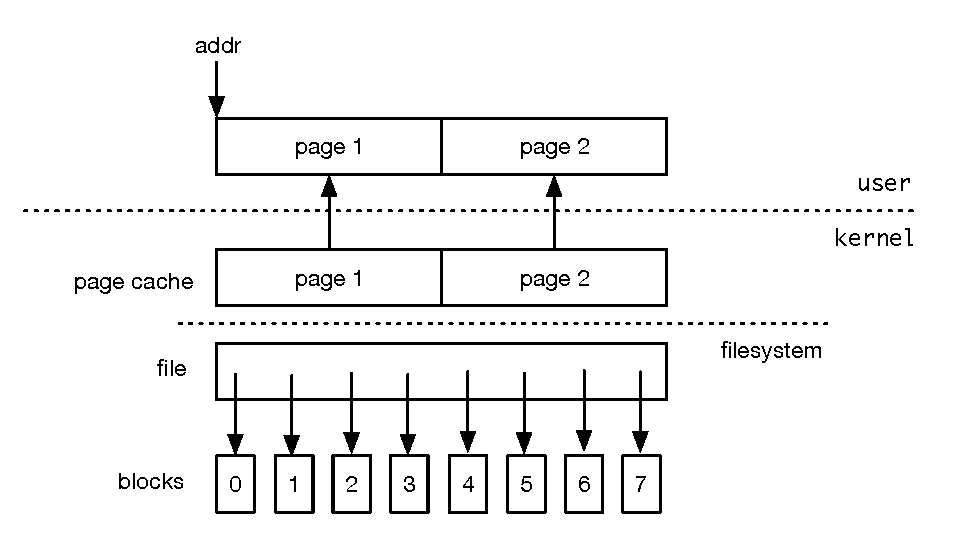
\includegraphics[scale=0.6]{figures/mmap-example.pdf}
	\centering
	\caption{Mapping an 8 KB file into memory}
	\label{fig:mmap-example}
\end{figure}

As we walk through the mapping, the kernel will call the filesystem to bring data into memory. This data is cached in the Linux page cache in the kernel. Here, two pages are allocated. Data is then copied from the kernel pages into the user pages starting at address \cf{addr}. If we run the program again, it is very likely that the pages in the Linux page cache will still be present so no more I/O will take place.

%------------------------------------------------------------------------------------------------------------------------------------------------------------------------

\subsection{The \cf{mmap(2)} / \cf{munmap()} System Calls}

The definition of \cf{mmap(2)} and \cf{munmap(2)} are as follows:

\begin{lstlisting}
void *mmap(void *addr, size_t length, int prot, int flags,
           int fd, off_t offset);
			  
int   munmap(void *addr, size_t length);
\end{lstlisting}

\noindent
The \cf{addr} argument is a hint as to where the region of the file will be mapped in memory. It must be correctly aligned according to the architecture on which the process is running. A page-aligned address should be used. The \cf{prot} argument specifies the memory protection of the mapping and can be one of the following:

\begin{itemize}
	\item \cf{PROT\_EXEC} -- pages may be executed.
	\item \cf{PROT\_READ} -- pages may be read.
	\item \cf{PROT\_WRITE} -- pages may be written.
	\item \cf{PROT\_NONE} -- pages may not be accessed.
\end{itemize}

\noindent
The \cf{flags} argument can be one of 20 different values. A few of the more widely used flags are:

\begin{itemize}
	\item \cf{MAP\_SHARED} -- the mapping can be shared with other processes .  Updates to the mapping are visible to other
              processes  mapping  the  same  region of the file, and changes made by any process are carried through to the 
              underlying  file.
	\item \cf{MAP\_PRIVATE} -- create a private copy-on-write mapping.  Any updates to the  mapping
              are  not  visible  to other processes mapping the same part of the file, and are not carried through to the underlying file.  
	\item \cf{MAP\_FIXED} -- don't interpret \cf{addr} as a hint and place  the  mapping  at  exactly the address specified 
		by \cf{addr}.
\end{itemize}

\noindent
The \cf{fd} argument specifies the file to be mapped and the \cf{offset} argument is an offset within the file. It should be a multiple of the system's page size.

The \cf{munmap(2)} system call can be called to delete the mapping for the specified address range (\cf{addr} and \cf{length}. Subsequent references to addresses within the range being unmapped will generate \cf{SIGSEGV}.  The  \cf{addr} argument must be a multiple of the page size (but the \cf{length} argument need not  be).   

%------------------------------------------------------------------------------------------------------------------------------------------------------------------------

\subsection{Other Mapped File Functions}

There are several other functions related to file mappings that are highlighted below:

\begin{itemize}
	\item \cf{msync(2)} -- flush changes made to the mapping back to the underlying file. An address and length are specified
		with flags indicating whether to perform writes synchronously, asynchronously and whether to invalidate any other  	
		mappings of the file so that subsequent access will bring in the new changes from disk.
	\item \cf{mlock(2)} / \cf{mlock2(2)} \cf{mlockall(2)} -- lock a number or all pages into memory to prevent them from
		being written to swap. A call to \cf{mlock2(2)} differs only if a flag of \cf{MLOCK\_ONFAULT} is specified in
		which case resident pages are locked and if pages within the mapping are current paged out, they will be 
		locked once they are faulted back into memory.
	\item \cf{mprotect(2)} -- when a call to \cf{mmap(2)} is made, the \cf{prot} argument specifies the access protections
		(for example \cf{PROT\_READ} or \cf{PROT\_READ}. This call allows those protections to be changed for an
		existing mapping. There are some additional access protections that are not part of the original \cf{mmap(2)}
		system call.
	\item \cf{mremap(2)} -- expands or shrinks an existing memory mapping and potentially moving the mapping at the same time
		depending on what flags are specified.
\end{itemize}
       
\noindent
Executables and corresponding libraries can be very large and it's unknown as to how much of the program binary will be used. The best method of reducing memory usage and I/O is to use \textit{demand paging}. The loader will establish a mapping to the executable as well as the various dynamic libraries that the program is linked with. When the process starts executing it will only bring in pages that are accessed. To further reduce memory, the mappings to program binaries and libraries are shared between processes. Program executables only need read access.

%%%%%%%%%%%%%%%%%%%%%%%%%%%%%%%%%%%%%%%%%%%%%%%%%%%%%%%%%%%%%%%

\section{Asynchronous I/O}

The \cf{read(2)} and \cf{write(2)} system calls are synchronous, that is, each operation will not return until the data is read/written or an error condition occurs. Depending on the type of I/O, the Linux kernel may have to call the filesystem which may have to go to disk to complete the operation. This is a time-consuming task compared to what an application could be doing if it solely operated on data in memory. While vectored reads/writes allow multiple I/Os to take place during a single call, likely improving performance, the application will still pause until the operation completes. Further optimizations can take place with threads which we will discuss in the next section. But prior to the widespread availability of \textit{pthreads} (process threads), asynchronous I/O, commonly called async I/O, was introduced whereby I/O operations could be started and the application would be notified asynchronously at a later time when the operation(s) completes. This allows the application to perform other tasks. One of the main drivers for async I/O, were the commercial databases such as Oracle. 

The \cf{aio(7)} manpage describes the different async I/O functions available. There is quite a lot to explain about these functions, but starting with the read/write interfaces:

\begin{lstlisting}
#include <aio.h>

int aio_read(struct aiocb *aiocbp);
int aio_write(struct aiocb *aiocbp);
int lio_listio(int mode, struct aiocb *restrict const 
               aiocb_list[restrict], int nitems, 
               struct sigevent *restrict sevp);
\end{lstlisting}

\noindent
The first two functions initiate single read/write operations while \cf{lio\_listio(3)} initiates the list of I/O operations described by the array \cf{aiocb\_list}. The \cf{aiocb} structure (aync I/O control block or AIO control block) contains the parameters used to specify the I/O operation or operations. It is defined in the \cf{aiocb.h} header file as follows:

\begin{lstlisting}
struct aiocb {
   int             aio_fildes;     /* File descriptor */
   off_t           aio_offset;     /* File offset */
   volatile void  *aio_buf;        /* Location of buffer */
   size_t          aio_nbytes;     /* Length of transfer */
   int             aio_reqprio;    /* Request priority */
   struct sigevent aio_sigevent;   /* Notification method */
   int             aio_lio_opcode; /* Operation to be performed; 
                                      lio_listio() only */                                     
}
\end{lstlisting}

\noindent
The first four fields will be recognizable as they are similar the arguments that would be passed to \cf{pread(2)} or \cf{pwrite(2)} so basically a call to \cf{lseek(2)} followed by a read or write. The \cf{aio\_reqprio} field specifies the relative priority of the I/O request. If the process priority is X and \cf{aio\_reqprio} is 6, the resulting priority of the I/O task is 10 - 6 = 4. \textbf{XXX--- need to come back to this}

\cf{aio\_lio\_opcode} is used by \cf{lio\_listio(3)} only and can be one of the following depending on what the operation is to perform:

\begin{lstlisting}
enum { LIO_READ, LIO_WRITE, LIO_NOP };
\end{lstlisting}

\noindent
The \cf{lio\_listio(3)} function can perform a mix of reads and writes with a single call. By setting  \cf{aio\_lio\_opcode} is set to \cf{LIO\_NOP} that specific AIO control block is ignored. 

The \cf{aio\_sigevent} specifies the mechanism through which the application is notified when the async I/O operation completes.

\begin{lstlisting}
struct sigevent {
    int             sigev_notify; /* Notification type */
    int             sigev_signo;  /* Signal number */
    union sigval    sigev_value;  /* Signal value */
    void          (*sigev_notify_function)(union sigval);
                                  /* Notification function */
    pthread_attr_t *sigev_notify_attributes;
                                  /* Notification attributes */
};
\end{lstlisting}

\noindent
I won't go into the details of each field of this structure but the example below will show how it is used. Refer to the \cf{sigevent(7)} manpage for more information.

To demonstrate how async I/O works in practice, we will givean example of how to issue multiple async I/Os to the same but using the \cf{lio-listio()} function. Figure \ref{fig:asyncio} shows a file contains 10 \cf{0}s followed by 10 \cf{1}s, 10 \cf{2}s and so on. Our goal is to read the \cf{1}s in an area of memory referenced by \cf{buf1}, overwrite the \cf{2}s with the contents of the memory referenced by \cf{buf2} and read the \cf{3}s in an area of memory referenced by \cf{buf3}.

\begin{figure}
	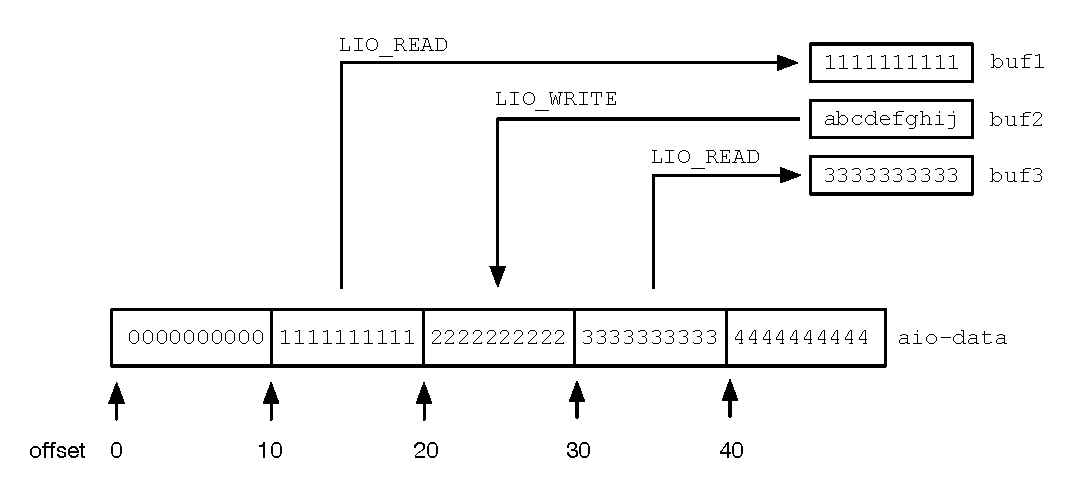
\includegraphics[scale=0.6]{figures/asyncio.pdf}
	\centering
	\caption{Reading and writing from/to a file using async I/O}
	\label{fig:asyncio}
\end{figure}

Most of the program involves setting up our three AIO control blocks which we do in lines 31-45 after opening our file \cf{aio-data}.

\begin{lstlisting}
 1 #include <fcntl.h>
 2 #include <aio.h>
 3 #include <signal.h>
 4 #include <stdio.h>
 5 #include <string.h>
 6 #include <unistd.h>
 7 #include <sys/uio.h>
 8 
 9 char *buf2 = "abcdefghij";
10 char buf1[32];
11 char buf3[32];
12 
13 void
14 aio_hdlr(int signo)
15 {
16     printf("buf1 = %.10s\n", buf1);
17     printf("buf3 = %.10s\n", buf3);
18 }
19 
20 int
21 main(int argc, char *argv[])
22 {
23     struct sigaction act;
24     struct sigevent  sevp;
25     struct aiocb     *list_aio[3];
26     struct aiocb     aio1, aio2, aio3;
27     int              err, fd;
28 
29     fd = open("aio-data", O_RDWR);
30 
31     aio1.aio_fildes  = fd;   aio1.aio_lio_opcode = LIO_READ;
32     aio1.aio_buf     = buf1; aio1.aio_offset     = 10;
33     aio1.aio_nbytes  = 10;   aio1.aio_reqprio    = 0;
34 
35     aio2.aio_fildes  = fd;   aio2.aio_lio_opcode = LIO_WRITE;
36     aio2.aio_buf     = buf2; aio2.aio_offset     = 20;
37     aio2.aio_nbytes  = 10;   aio2.aio_reqprio    = 0;
38 
39     aio3.aio_fildes  = fd;   aio3.aio_lio_opcode = LIO_READ;
40     aio3.aio_buf     = buf3; aio3.aio_offset     = 30;
41     aio3.aio_nbytes  = 10;   aio3.aio_reqprio    = 0;
42 
43     list_aio[0] = &aio1;
44     list_aio[1] = &aio2;
45     list_aio[2] = &aio3;
46 
47     memset(&act, 0, sizeof(act));
48     act.sa_handler = aio_hdlr;
49     sigaction(SIGUSR1, &act, NULL);
50     act.sa_handler = SIG_IGN;
51     sigaction(SIGHUP, &act, NULL);
52 
53     memset(&sevp, 0, sizeof(sevp));
54     sevp.sigev_signo = SIGUSR1;
55     sevp.sigev_notify = SIGEV_SIGNAL;
56     sevp.sigev_value.sival_ptr = (void *)list_aio;
57 
58     err = lio_listio(LIO_NOWAIT, list_aio, 3, &sevp);
59     pause();
60 }
\end{lstlisting}

\noindent
\textbf{XXX---need to either explain the issue with SIGHUP or fix it!!! - also, perhaps we can have the signal handler analyze the aiocbs (re sigevent) otherwise all that stuff on 53-56 is kind of wasted}

Additional info about the program is as follows:

\begin{itemize}
	\item Lines 47 - 51 -- When the async I/O operations complete the program will be notified by a signal. 
		I'm choosing \cf{SIGUSR1} as the signal to use and my signal handler is the function \cf{aio\_hdlr}.
		Lines 47 - 49 provide the set up needed. \textbf{XXX---SIGHUP dunno}
	\item Lines 53 - 56 -- \cf{lio\_listio(3)} requires a pointer to a \cf{sigevent} structure which tells it which
		signal to post and a pointer to a structure which will be passed to the signal handler. This allows
		the program to check for the status of individual I/O operations. For more details about how async I/O
		uses signal handler, refer to the \cf{sigevent(7)} manpage.
	\item Line 58 -- Call \cf{lio\_listio(3)} to initiate the I/O operations.
	\item Line 59 -- Pause the program to wait for signal handling. Once the signal handler runs, 
		\cf{pause(2)} returns and the program will exit.
\end{itemize}

\noindent
Before running the program, we display the contents of the \cf{aio-data} file, then run the program and then display the file contents again. As you can see, \cf{buf1} and \cf{buf2} contain the data expected and \cf{aio-data} is overwritten at offset 20 with the string \cf{abcdefghij} referenced by \cf{buf2}.

\begin{lstlisting}
$ [*\bfseries cat aio-data*]
00000000001111111111222222222233333333334444444444
$ [*\bfseries ./aio*]
buf1 = 1111111111
buf3 = 3333333333
$ [*\bfseries cat aio-data*]
00000000001111111111abcdefghij33333333334444444444
\end{lstlisting}

%----------------------------------------------------------------------------------------------------------------------------------------------------------------

\subsection{Additional Async I/O Functions}

There are several other functions available that are needed to build enterprise applications and worth exploring. They are highlighted below. Also, view the \cf{aio(7)} manpage for additional information.

\begin{itemize}
       \item \cf{aio\_fsync(3)} --- Queue a \textit{sync} request for the I/O operations on the file descriptor specified
       		in the AIO control block. This is somewhat equivalent to calling of \cf{fsync(2)} and \cf{fdatasync(2)}. 
		If the \cf{op} argument is \cf{O\_SYNC}, then all currently queued I/O operations shall 
		be completed as if by making a call to \cf{fsync(2)}, and if \cf{op} is \cf{O\_DSYNC}, this call is the 
		asynchronous analog of \cf{fdatasync(2)}. This function doesn't wait for I/Os to completion.

       \item \cf{aio\_error(3)} --- Obtain  error status of a queued I/O request.

       \item \cf{aio\_return(3)} --- Obtain the return status of a completed I/O request.

       \item \cf{aio\_suspend(3)} --- Suspend the caller until one or more of a specified set of I/O requests completes.

       \item \cf{aio\_cancel(3)} --- Attempt to cancel outstanding I/O requests on a specified file descriptor.
\end{itemize}

%%%%%%%%%%%%%%%%%%%%%%%%%%%%%%%%%%%%%%%%%%%%%%%%%%%%%%%%%%%%%

\subsection{Performance Gains with Async I/O}

Disks have come a long way since the POSIX async I/O standard was being developed back in the early 1990s. But even with  faster disks, disk subsystems and SSDs, it's still slow to \textit{go to disk} compared with reading from an in-core cache, whether the Linux page cache or a database cache. Also recall that at the time of the async I/O standard being developed, CPU cores were non-existent and the multi-threading standard known as pthreads was still being developed. When I was at ICL (International Computers Limited), we were implementing async I/O on SVR4 UNIX implementation on top of the Chorus microkernel to support Oracle. I recall the performance gains made by the database to be huge although it was a long time ago so I don't recall the details.

\begin{quote}
You don't have to worry about threading or race conditions or losing error state (as much). AFIO does all that for you.
On platforms which provide native asynchronous file i/o support and/or native scatter/gather file i/o support, AFIO will use that instead of issuing multiple filing system operations using a thread pool to achieve concurrency. This can very significantly reduce the number of threads needed to keep your storage device fully occupied — remember that queue depth i.e. that metric you see all over storage device benchmarks is the number of operations in flight at once, which implies the number of threads needed. Most storage devices are IOPS limited due to SATA or SAS connection latencies without introducing queue depth — in particular, modern SSDs cannot achieve tens of thousands of IOPS range without substantial queue depths, which without using a native asynchronous file i/o API means lots of threads.
It's very, very easy to have AFIO turn off file system caching, readahead or buffering on a case by case basis which makes writing scalable random synchronous file i/o applications much easier.
\end{quote}

\textbf{XXX---need to come back and enhance once the FS performance chapter is finished}

Oracle but any info? Not easy to find.

Lighty - http://blog.lighttpd.net/articles/2006/11/12/lighty-1-5-0-and-linux-aio/ 

wikipedia - %https://en.wikipedia.org/wiki/Asynchronous_I/O 

just search for "application+performance+gains+examples" - there are lots of examples

%----------------------------------------------------------------------------------------------------------------------------------------------------------------

\subsection{procfs Async I/O Information}

There are two files in the proc file system that can be tuned for asynchronous I/O. Both can be found under \cf{/proc/sys/fs}:

\begin{itemize}
	\item \cf{aio-nr} --- the current number of system-wide asynchronous I/O requests. If there are no
		async I/O requests active, this number will be 0.
	\item \cf{aio-max-nr} --- the maximum number of allowable concurrent requests. This is generally 64 KB.
\end{itemize}

%%%%%%%%%%%%%%%%%%%%%%%%%%%%%%%%%%%%%%%%%%%%%%%%%%%%%%%%%%%%%

\section{Truncating Files}\label{prog-truncate}

When describing the \cf{open(2)} system call in section \ref{prog-open-flags}, the \cf{O\_TRUNC} flag can be passed to ensure that the file is truncated to length of zero if the file already exists. If a file needs to be truncated either without opening it or after the file is opened, the following system calls can be used:

\begin{lstlisting}
#include <unistd.h>

int truncate(const char *path, off_t length);
int ftruncate(int fd, off_t length);
\end{lstlisting}

\noindent
The difference between using \cf{O\_TRUNC} during a call to \cf{open(2)} and the above interfaces is that the file will be truncated to exactly \cf{length} bytes.

A file can be truncated down in size or it can be truncated up. I always found that amusing when I very first saw this descriptioin many years ago. How do you allocate space to a file? "Truncate the file up"!

If the size of the file is larger than the size specified by \cf{length}, the extra data will be lost following the truncation.  If the file is shorter, it will be is extended. The extended part will read as null bytes ('\cf{\textbackslash0'}).

%%%%%%%%%%%%%%%%%%%%%%%%%%%%%%%%%%%%%%%%%%%%%%%%%%%%%%%%%%%%%

\section{Multi-threaded Applications}

There have been several books written about multi-threaded applications and for the most part, multi-threading is beyond the scope of this chapter. The following web page gives a very good introduction into multi-threading and introduces not just multi-threading concepts but also pthreads, POSIX threads, the default method of multi-threading on Linux.

\begin{table}[h]
\begin{tabular}{lcl}
\parbox[r]{0.5in}{
\includegraphics[scale=0.15]{figures/url.png}} & \parbox[l]{0.55in}{URL \arabic{urls}} & \parbox[l]{3in}{\cf{https://tinyurl.com/5ssbe8db}}
\end{tabular}
\end{table}
\stepcounter{urls}
% https://randu.org/tutorials/threads/

\noindent
The \cf{pthreads(7)} manpage is the place to start to learn about the programming interfaces available that underpin pthreads. Over the last twenty years, Linux has seen two different implementations for pthreads:

\begin{itemize}
	\item LinuxThreads -- the original Pthreads implementation which, since glibc  2.4, is no longer supported.
	\item NPTL (Native POSIX Threads Library) -- the modern pthreads implementation.  By comparison with
              LinuxThreads, NPTL provides closer conformance to  the  requirements  of  the POSIX.1 specification than 
              LinuxThreads. It also has better performance when creating large numbers of  threads.  NPTL  has been 
              available  since glibc 2.3.2, and requires features that are present since the Linux 2.6 kernel.
\end{itemize}

\noindent
Start with \cf{pthreads(7)} and go from there. Most articles on line will reference the newer implementation. The \cf{getconf(1)} command can be used to determine which implementation is available:

\begin{lstlisting}
$ [*\bfseries getconf GNU\_LIBPTHREAD\_VERSION*]
NPTL 2.36
\end{lstlisting}

\noindent
When developing applications that access files / filesystems, there aren't many things to bear in mind when writing multi-threaded applications:

\begin{itemize}
	\item All open files are shared between all process threads. If a thread (other than \cf{main()}) opens a file, it should 
		be closed before the thread terminates.
	\item Linux file locking has issues when deploying multi-threaded applications. Please refer to section \ref{prog-locking}
		and make sure you use the newer \textit{Open File Description Locks}. 
	\item It should go without saying that any change that any thread makes, including calls resulting in a state change
		in the kernel, are visible to all other threads. Since file descriptors are shared, offsets within each file are
		also shared.
\end{itemize}

%%%%%%%%%%%%%%%%%%%%%%%%%%%%%%%%%%%%%%%%%%%%%%%%%%%%%%%%%%%%%

\section{Directory Creation}\label{prog-mkdir}

Directory creation is handled by the \cf{mkdir(2)} and \cf{mkdirat(2)} system calls:

\begin{lstlisting}
#include <sys/stat.h>

int mkdir(const char *pathname, mode_t mode);

#include <fcntl.h>           /* Definition of AT_* constants */ 
#include <sys/stat.h>

int mkdirat(int dirfd, const char *pathname, mode_t mode);
\end{lstlisting}

\noindent
For \cf{mkdir(2)}, the pathname can be absolute or relative. The \cf{mode} argument specifies the mode for the newly created directory. It is modified by the process's umask using the formula (\cf{mode \& \~{}umask \& 0777}).

How the \cf{mkdirat(2)} system call operates depends on \cf{pathname}. Either:

\begin{itemize}
	\item If \cf{pathname} is relative, it is interpreted relative to the directory referred to  by  the  file  descriptor  \cf{dirfd}
		as opposed to being relative to the current working directory of the calling process (as is done by \cf{mkdir(2)} 
		for a relative pathname).
	\item If \cf{pathname} is relative and \cf{dirfd} is set to \cf{AT\_FDCWD},  \cf{pathname} is interpreted relative to 
		the current working directory of the calling process (as for \cf{mkdir(2)}).
	\item If \cf{pathname} is absolute, \cf{dirfd} is ignored.
\end{itemize}

\noindent
Removing a directory is very straightforward:

\begin{lstlisting}
#include <unistd.h>

int rmdir(const char *pathname);
\end{lstlisting}

\noindent
The directory must be empty before this operation can succeed.

%%%%%%%%%%%%%%%%%%%%%%%%%%%%%%%%%%%%%%%%%%%%%%%%%%%%%%%%%%%%%

\section{Hard Links and Symbolic Links}\label{prog-links}

Creating a hard link with the \cf{link(2)} or \cf{linkat(2)} system calls involves creation of a new directory entry that references the file to which it is linked to. Following a successful call, the file referenced by \cf{newpath} can be used in exactly the same manner as the file \cf{oldpath}, to which it is linked.

\begin{lstlisting}
#include <unistd.h>

int link(const char *oldpath, const char *newpath);

#include <fcntl.h>           /* Definition of AT_* constants */ 
#include <unistd.h>

int linkat(int olddirfd, const char *oldpath,
           int newdirfd, const char *newpath, int flags);
\end{lstlisting}

\noindent
Below is a simple example showing the effects of calling \cf{link(2)}. All the program does is create a hard link called "\cf{latin-text}" to the existing file "\cf{lorem-ipsum}".

\begin{lstlisting}
#include <unistd.h>

int
main()
{
    link("lorem-ipsum", "latin-text");
}
\end{lstlisting}

\noindent
Before the program is run, the attributes of "\cf{lorem-ipsum}" are displayed. The link count for this file is "1". The program is then run and the link count goes to "2". When the attributes of "\cf{latin-text}", you can see they mirror the attributes of "\cf{lorem-ipsum}".

\begin{lstlisting}
$ [*\bfseries ls -li lorem-ipsum *]
409993 -rw-r--r-- [*\bfseries 1*] spate spate 2972 Apr  4 16:43 lorem-ipsum
$ [*\bfseries ./link*]
$ [*\bfseries ls -li lorem-ipsum*] 
409993 -rw-r--r-- [*\bfseries 2*] spate spate 2972 Apr  4 16:43 lorem-ipsum
$ [*\bfseries ls -li latin-text  *]
409993 -rw-r--r-- [*\bfseries 2*] spate spate 2972 Apr  4 16:43 latin-text
$ [*\bfseries diff lorem-ipsum latin-text  *]
\end{lstlisting}

\noindent
The \cf{linkat(2)} system call differs from \cf{link(2)} primarily in how the two files are referenced. See the previous section on how \cf{mkdirat(2)} operates. The main difference here is that there is an additional \cf{flags} argument which can be a bitwise OR of the following:

\begin{itemize}
	\item \cf{AT\_EMPTY\_PATH} -- If \cf{oldpath} is an empty string then the link will be created to reference the file
		\cf{olddirfd}.
	\item \cf{AT\_SYMLINK\_FOLLOW} -- By default, \cf{oldpath} will not be dereferenced if it is a symbolic  link, the same
		being is true with \cf{link(2)}).  If \cf{AT\_SYMLINK\_FOLLOW} is specified in \cf{flags} and \cf{oldpath} is a symbolic 
		link, it will be dereferenced.
\end{itemize}

\noindent
The \cf{unlink(2)} and  \cf{unlinkat(2)} system calls can be used to remove a link to a file:

\begin{lstlisting}
#include <unistd.h>

int unlink(const char *pathname);

#include <fcntl.h>           /* Definition of AT_* constants */
#include <unistd.h>

int unlinkat(int dirfd, const char *pathname, int flags);
\end{lstlisting}

\noindent
 If \cf{pathname} is the last link to a file and no processes have the file open, the file will deleted and any space it is using will be reclaimed and made available for other use. If \cf{pathname} references a symbolic link, only the link is removed.
 
 The \cf{unlinkat(2)} system call operates the same way as both \cf{unlink(2)} and \cf{rmdir(2)}. If the \cf{flag} argument is \cf{AT\_REMOVEDIR}, the equivalent of \cf{rmdir(2)} will be performed.
 
%%%%%%%%%%%%%%%%%%%%%%%%%%%%%%%%%%%%%%%%%%%%%%%%%%%%%%%%%%%%
 
 \subsection{Symbolic Links}
 
The \cf{symlink(2)} system call creates a symbolic link called \cf{linkpath}. It will contain the string \cf{target}. The existence of the target file is not checked during this operation.
 
\begin{lstlisting}
#include <unistd.h>

int symlink(const char *target, const char *linkpath);

#include <fcntl.h>           /* Definition of AT_* constants */ 
#include <unistd.h>

int symlinkat(const char *target, int newdirfd, 
              const char *linkpath);
\end{lstlisting}

\noindent
The \cf{symlinkat(2)} system call operates in the same way as \cf{symlink(2)} with the following two exceptions:

\begin{itemize}
	\item If \cf{linkpath} is relative, it will be interpreted relative to the directory referred to by the file descriptor \cf{newdirfd}.
	\item If  \cf{linkpath} is relative and \cf{newdirfd} is the value \cf{AT\_FDCWD}, \cf{linkpath} is interpreted relative to the 
		current working directory of the calling process (like symlink()).
\end{itemize}

%%%%%%%%%%%%%%%%%%%%%%%%%%%%%%%%%%%%%%%%%%%%%%%%%%%%%%%%%%%%%

\section{Extended Attributes}

A file contains both the regular stream of data as written by applications in addition to meta-data created and maintained by the filesystem. User-visible meta-data can be obtained by running one of the \cf{stat(2)} system calls. Application developers pushed the operating system and small number of filesystem vendors for years to have them store user-defined attributes. As a specific example, back in the early to mid 1990s, I used to be a member of DMIG (the Data Management Interfaces Group) who were building storage management APIs to support Hierarchical Storage Management (HSM) applications. To save space on disk storage, HSM applications would punch holes in files accessed less frequently and store that data on tape to be read back at a later time when the file was accessed. This was a complex process and required per-file meta-data about the data being migrated to tertiary storage. At this time few vendors support such \textit{extended attributes}. But this was the beginning of what would become a POSIX standard. 

Today, the following filesystems in Linux support extended attributes---ext2, ext3, ext4, JFS, XFS, btrfs, OCFS2 and squashfs. Extended attributes have a name and associated data. Attribute names can be up to 255 characters and the size of the associated data is variable depending on the filesystem.

Linux provides four namespaces for extended file attributes:

\begin{enumerate}
	\item user
	\item trusted
	\item security
	\item system
\end{enumerate}

\noindent
The name of the attribute must start with one of the four names shown above followed a "." and then followed an application supplied name. An example could be \cf{user.comment}. The \cf{xattr(2)} manpage contains details about the different extended attribute system calls and commands. The \cf{setfattr(1)} and \cf{getfattr(1)} commands can be used to set and get extended attribute. The systems calls are \cf{setxattr(2)}, \cf{getxattr(2)}, \cf{removexattr(2)} and \cf{listxattr(2)} (which is used by "\cf{getfattr -d}").

\subsection{Installing and Using Extended Attributes}

On Ubuntu you need to install the \cf{attr} package as follows:

\begin{lstlisting}
$ [*\bfseries sudo apt install attr*]
\end{lstlisting}

\noindent
in order to start using extended attributes. In the example below, \cf{ls} is run against the file "\cf{lorem-ipsum}", an attribute is added and then \cf{ls} is run again. You'll see that the file looks exactly the same.

\begin{lstlisting}
$ [*\bfseries ls -l lorem-ipsum*]
-rw-r--r-- 1 spate spate 2972 Dec  4 15:43 lorem-ipsum
$ [*\bfseries setfattr -n user.comment -v "File contains Latin" lorem-ipsum*]
$ [*\bfseries ls -l lorem-ipsum*]
-rw-r--r-- 1 spate spate 2972 Dec  4 15:43 lorem-ipsum
\end{lstlisting}

\noindent
Extended attributes stored in a file can bee read the contents as follows:

\begin{lstlisting}
$ [*\bfseries getfattr -d lorem-ipsum*]
# file: lorem-ipsum
user.comment="File contains Latin"
\end{lstlisting}

\noindent
Despite demand for extended attributes over the years, their adoption has been somewhat limited. On Linux, The Wikipedia page on extended attributes mentions that they are used by Beagle, OpenStack Swift, Dropbox, KDE's semantic metadata framework (Baloo), Chromium, Wget and cURL. Desktop file manager usage has always been one of the most quoted examples but generally speaking, unless all underlying filesystems support extended attributes, the presentation to the user becomes more difficult to implementers since they can use extended attributes where available but then must use some other mechanism for storing attributes if the underlying filesystem does not support them. This results in a less than stellar presentation or an awkward implementation.

%%%%%%%%%%%%%%%%%%%%%%%%%%%%%%%%%%%%%%%%%%%%%%%%%%%%%%%%%%%%%

\section{Inode Flags}

Some of the Linux filesystems support the notion of \textit{inode flags} which are described in the \cf{ioctl\_iflags(2)} manpage. Inode flags are attributes used to modify the semantics of files and directories. These flags can be retrieved and modified using the following two \cf{ioctl(2)} operations:

\begin{lstlisting}
int attr, fd;

fd = open("filename", ...);
ioctl(fd, FS_IOC_GETFLAGS, &attr);  // get current flags
attr |= FS_NOATIME_FL;              // set the flags you want
ioctl(fd, FS_IOC_SETFLAGS, &attr);  // update the file's flags
\end{lstlisting}

\noindent
The first call retrieves the current flags and puts then in \cf{attr}. The bitmask is then modified and a second call is made to set the new flags. There are 14 flags in total and changes apply even if the caller has superuser privileges. Here are a few of the available flags:

\begin{itemize}
	\item \cf{FS\_APPEND\_FL} --  prevent the file from being opened only with  \cf{O\_APPEND}.
	\item \cf{FS\_IMMUTABLE\_FL} -- the file will be set to be immutable; no subsequent changes can be made to the 
		file contents or metadata.
	\item \cf{FS\_SYNC\_FL} -- make all future writes synchronous.
	\item \cf{FS\_NOATIME\_FL} -- the file's access time (atime) will not be update on access. This can have significant
		performance benefits.
\end{itemize}

\noindent
Inode flags are Linux specific, not part of any standard and not implemented by all of the Linux filesystems.

%%%%%%%%%%%%%%%%%%%%%%%%%%%%%%%%%%%%%%%%%%%%%%%%%%%%%%%%%%%%%

\section{Reading Directory Entries}\label{prog-readdir}

As you will see later in the book, parsing pathnames and handling directory entries is a complex task for both the kernel and filesystems to handle. In fact, supporting a very large number of files inside a single directory is a particularly complex task for filesystem developers.

Reading directory entries is performed by the \cf{readdir(3)} library function which is passed a \cf{DIR} structure, called a \textit{directory stream}, obtained from calling \cf{opendir(3)}. Both functions are defined as follows:

\begin{lstlisting}
#include <sys/types.h>
#include <dirent.h>

DIR *opendir(const char *name);
DIR *fdopendir(int fd);
int closedir(DIR *dirp);

struct dirent *readdir(DIR *dirp);
\end{lstlisting}

\noindent
For \cf{opendir(3)}, the \cf{name} argument should reference a directory either as a relative or absolute pathname. On return, the directory stream will be positioned ready to read the first entry in the directory. The \cf{fopendir(3)} library function also returns a directory stream but using a specified file descriptor. Note that the file descriptor should not be used for any other operation. The \cf{closedir(3)} function closes the directory stream as well as the underlying file descriptor.

Given a directory stream, an application can make calls to \cf{readdir(3)} with each call returning the next directory entry with each entry defined by the \cf{dirent} structure. I've only included three of the fields of this structure. Only the first two fields are required by POSIX. In the following section, I'll show an example of a simple version of the \cf{ls(1)} command which uses the first two fields but then uses the \cf{lstat(2)} system call to get the file type.

\begin{lstlisting}
struct dirent {
    ino_t          d_ino;       /* Inode number */
    char           d_name[256]; /* Null-terminated filename */
    unsigned char  d_type;      /* Type of file */
};
\end{lstlisting}

\noindent
Once all directory entries have been returned, the return value will be \cf{NULL}. You should not make any assumption about the order in which directory entries are returned. This will likely different from one filesystem to the next. 

%------------------------------------------------------------------------------------------------------------------------------------------------------------------------

\subsection{A Simple Implementation of the \cf{ls(1)} Command}\label{ls-command}

To give an example of how \cf{readdir(3)} can be used, here is a simple version of the \cf{ls(1)} command which does the equivalent of \cf{ls -al} on the current directory. The source code to our minimal \cf{ls} command is shown below. For the \cf{print\_*} functions, the source code is available at the book's github site. There is a fair amount of processing of the \cf{stat} structure, mapping between UID/GID and actual string representations and manipulation of the modification time to get it into the right format. 

\begin{lstlisting}
 1 int
 2 main() {
 3     struct dirent *dir;
 4     DIR           *mydir;
 5     struct stat   st;
 6  
 7     mydir = opendir(".");
 8     while (1) {
 9         dir = readdir(mydir);
10         if (dir == NULL) {
11             break;
12         }
13         lstat(dir->d_name, &st);
14         print_file_type(&st);
15         print_perms(&st);
16         printf(" %d ", st.st_nlink);
17         print_owner_group(&st);
18         printf("%5ld ", st.st_size);
19         print_mtime(&st);
20         printf("%s\n", dir->d_name);
21     }
22 }
\end{lstlisting}

\noindent
The program is quite simple, looping through the directory making calls to \cf{readdir(3)} (line 9) to read each directory entry. Once the last entry has been read, \cf{NULL} will be returned. Then for each directory entry read, we print out the various fields to match the output returned by running \cf{ls -al}.

As mentioned above, the \cf{d\_type} field of the \cf{dirent} structure is not POSIX compliant but could be used to avoid a call to \cf{lstat(2)}. In our example, we want more information about the file so this call is necessary. Furthermore, we need to call \cf{lstat(2)} in place or \cf{stat(2)} since, if this was a symbolic link, we would information about the symbolic link and not the file to which it points to.

The \cf{print\_file\_type()} function simply checks the \cf{S\_IFMT} field of the \cf{stat} structure. Here is a fragment of the source code:

\begin{lstlisting}
print_file_type(struct stat *st)
{
    char c;

    switch (st->st_mode & S_IFMT) {
        case S_IFBLK:
            c = 'b';
            break;
        case S_IFCHR:
            c = 'c';
            break;
        ...
        default:
            c = '?';
            break;
    }
    printf("%c", c);
}
\end{lstlisting}

\noindent
Below is output from the program running showing contents of a directory with several different file types followed by running the real \cf{ls -l}:

\begin{lstlisting}
$ [*\bfseries ./myls*]
brw-r--r-- 1 root  root      0 Dec 19 17:41 mydev
drwxrwxr-x 2 spate spate  4096 Dec 19 17:39 mydir
drwxrwxr-x 3 spate spate  4096 Dec 19 17:41 .
-rw-r--r-- 1 spate spate   325 Dec 19 17:39 sparse.c
prw-rw-r-- 1 spate spate     0 Dec 19 17:40 mypipe
drwxrwxr-x 4 spate spate  4096 Dec 19 19:41 ..
-rwxrwxr-x 1 spate spate 70504 Dec 19 17:39 fds
$ [*\bfseries ls -al*]
total 32
drwxrwxr-x 3 spate spate  4096 Dec 19 17:41 .
drwxrwxr-x 4 spate spate  4096 Dec 19 19:41 ..
-rwxrwxr-x 1 spate spate 70504 Dec 19 17:39 fds
brw-r--r-- 1 root  root   4, 5 Dec 19 17:41 mydev
drwxrwxr-x 2 spate spate  4096 Dec 19 17:39 mydir
prw-rw-r-- 1 spate spate     0 Dec 19 17:40 mypipe
-rw-r--r-- 1 spate spate   325 Dec 19 17:39 sparse.c
\end{lstlisting}

\noindent
The \cf{ls(1)} program does a lot of formatting. When you run \cf{ls -l}, the "." and ".." entries are displayed first. The spacing around the owner, group and file size are nicely done. This implies that \cf{ls} must make at least one pass through the list of directory entries before it starts printing anything. However, all entries are read using \cf{readdir(3)} and then a call is made to \cf{sort\_files()} to sort / format them. You can find the source code to the \cf{ls(1)} command here:

\begin{lstlisting}
https://github.com/wertarbyte/coreutils/blob/master/src/ls.c
\end{lstlisting}

\noindent
This simple version of \cf{ls} doesn't display the device file major/minor and won't nicely format directory entries if owner, group and size of more characters than those shown here.

%------------------------------------------------------------------------------------------------------------------------------------------------------------------------

\subsection{Other Directory Functions}

One of the most useful functions, and one which could simply our version of \cf{ls(1)} by getting an alphabetically sorted list of directory entries, is the \cf{scandir(3)}:

\begin{lstlisting}
#include <dirent.h>

int scandir(const char *restrict dirp,
           struct dirent ***restrict namelist,
           int (*filter)(const struct dirent *), 
           int (*compar)(const struct dirent **, 
                         const struct dirent **));
\end{lstlisting}

\noindent
The directory specified by \cf{dirp} is scanned and entries are sorted according to the function specified by \cf{comprar} which can be \cf{alphasort} which sorts directory entries using \cf{strcoll(3)}, or \cf{versionsort} which sorts using \cf{strverscmp(3)} on the strings \cf{(*a)->d\_name} and \cf{(*b)->d\_name}. As entries are being read, space is allocated by calling \cf{malloc(3)}. 

The \cf{filter} argument can be used to select specific entries. An an example, if our \cf{myls} program was given wildcards as an argument, the \cf{filter} function provided could be used to match specific files. If \cf{filter} is set to \cf{NULL} all directory entries will be returned. 

Here is a skeleton version of a program that we could have used for the \cf{myls} command above. Note that as we display each directory entry, we free the space that was allocated by \cf{scandir(3)}.

\begin{lstlisting}
#include <dirent.h>
#include <stdio.h>
#include <stdlib.h>

int
main(void)
{
   struct dirent **namelist;
   int nentries, i;

   nentries = scandir(".", &namelist, NULL, alphasort);
   for (i=0 ; i<nentries ; i++) {
       printf("%s\n", namelist[i]->d_name);
       free(namelist[i]);
   }
   free(namelist);

}
\end{lstlisting}

\noindent
Since we've passed \cf{alphasort} as an argument, we get all entries sorted nicely:

\begin{lstlisting}
$ [*\bfseries ./scandir*]
.
..
fds
mydev
mydir
mypipe
sparse.c
\end{lstlisting}

\noindent
There are other functions that allow you to browse directory trees which you can peruse at your own pleasure:

\begin{itemize}
	\item \cf{ftw(3)} --- Walk through a directory tree and calls the specified function for each entry in the tree.
	\item \cf{fts(3)} --- More functions for walking a directory tree.
	\item \cf{telldir(3)} --- Return current location in directory stream.
	\item \cf{seekdir(3)} --- Set the location in the directory  stream  from which  the next call to \cf{readdir(2)} 
		will start. A value returned by \cf{telldir(3)} should be used.
	\item \cf{rewinddir(3)} --- Reset the position of the directory stream to the beginning of the directory.
\end{itemize}

%------------------------------------------------------------------------------------------------------------------------------------------------------------------------

\subsection{Directory Entries at the System Call Level}

The library functions described in the sections above all build on top of a simple system call interface defined as follows in the \cf{getdents(2)} manpage:

\begin{lstlisting}
#include <sys/syscall.h>   /* Defn of SYS_* constants */
#include <unistd.h>

long syscall(SYS_getdents, unsigned int fd, 
             struct linux_dirent *dirp, unsigned int count);

#define _GNU_SOURCE.   /* See feature_test_macros(7) */
#include <dirent.h>

ssize_t getdents64(int fd, void *dirp, size_t count);
\end{lstlisting}

\noindent
As the manpage says:

\begin{quote}
\textit{These are not the interfaces you are interested in.  Look at readdir(3)
for the POSIX-conforming C library interface.  This page documents  the
bare kernel system call interfaces.}
\end{quote}

\noindent
If you browse the glibc source code, you'll see that it uses \cf{getdents64()} which returns one or more directory entries in the buffer pointed to by \cf{dirp}. The size of the buffer is referenced by \cf{count}. The number of entries read is returned and each entry returned is defined by the \cf{linux\_dirent} structure:

\begin{lstlisting}
struct linux_dirent64 {
    ino64_t        d_ino;    /* 64-bit inode number */
    off64_t        d_off;    /* 64-bit offset to next struct */
    unsigned short d_reclen; /* Size of this dirent */
    unsigned char  d_type;   /* File type */
    char           d_name[]; /* Filename (null-terminated) */
};
\end{lstlisting}

\noindent
Although it looks similar to \cf{readdir(3)} it requires a lot more work on behalf of the caller and thus the very large warning in the manpage. Applications should use the functions described earlier but it's important to highlight the system call since we will be describing its implementation later in the book in section \ref{vfs_readdir}.

%%%%%%%%%%%%%%%%%%%%%%%%%%%%%%%%%%%%%%%%%%%%%%%%%%%%%%%%%%%%%%%

\section{File Notification}\label{fanotify}

File notification is a mechanism where applications can be notified of events that occur within the filesystem in response to actions such a file creation, reads, writes and deletions.

There are several applications that can make use of filesystem notification events. Examples that come to mind are desktop file managers which can update their display of a directory as changes are made to the directory, malware scanners such as ClamAV and hierarchical storage management which is discussed elsewhere in the book. Another important example is backup. When determining what files to backup, scanning a filesystem looking for changes can be a time-consuming task. If the backup application already had a list of changed files, that scan could be avoided.

The three different file notification mechanisms that exist in Linux are as follows:

\begin{itemize}
	\item \textbf{dnotify} -- appearing in Linux in 2001, the first mechanism lacked the knowledge about how such frameworks
		should be used and relied on extensions to \cf{fcntl(2)}, for example "\cf{fcntl(fd, F\_NOTIFY, mask)}". Only
		directories could be monitored and not regular files. Delivery of a signal indicated notification of an event but the
		application needs to scan the directory to see what actually changed. There were additional shortcomings. 
	\item \textbf{inotify} -- first appearing in Linux 2.6.13 in 2005, the inotify framework intended to resolve the issues with
		dnotify. The three system calls, namely \cf{inotify\_init(2)}, \cf{inotify\_add\_watch(2)}, and \cf{inotify\_rm\_watch(2)}
		were introduced. An initialization call to \cf{inotify\_init(2)} returns a file descriptor which is used by the other
		inotify system calls. Files and directories can be added to the list of file objects to be monitored and the list and
		events could be added or removed. The \cf{inotify(7)} manpage lists all of the possible events. There are several
		advantages over dnotify. In additional to supporting regular files, the interface was simpler, there are more events
		and there is better information about each event received. For more details of inotify I recommend reading the
		lwn.net articles (search for "linux filesystem notification part".
	\item \textbf{fnotify} -- first appeared in Linux 2.6.37 in 2011 and will be described in this section. It has a superset
		of the inotify functionality. 
\end{itemize}

\noindent
With fanotify, it's possible to monitor a mounted filesystem as a whole unlike inotify. Despite being introduced in 2011, fanotify has seen several improvements over the years with major enhancements appearing in 2019 such as support for create, move, and delete events. These events were part of a \textit{directory events} addition at the time. 

Before describing how to use fanotify, there is an example  program at the following location that will be demonstrated here:

\begin{table}[h]
\begin{tabular}{lcl}
\parbox[r]{0.5in}{
\includegraphics[scale=0.15]{figures/url.png}} & \parbox[l]{0.55in}{URL \arabic{urls}} & \parbox[l]{3in}{\cf{https://tinyurl.com/2p9dmz2n}}
\end{tabular}
\end{table}
\stepcounter{urls}
% https://gist.github.com/jaypeche/497ac0c3ce36cdb7f5b9

\noindent
Note that you will likely need to replace the line that includes "\cf{linux/fanotify.h}" with the following:

\begin{lstlisting}
#include <sys/fanotify.h>
\end{lstlisting}

\noindent
To run the program, specify a directory (this example uses "\cf{mydir}") and events will be displayed as operations are performed on files within the specified directory:

\begin{lstlisting}
$ [*\bfseries sudo ./fanotify-example mydir*]
Started monitoring directory 'mydir'...
Received event in path '/home/spate/mydir/foo' pid=2813 (...): 
	FAN_OPEN
	FAN_CLOSE_WRITE
Received event in path '/home/spate/mydir/foo' pid=1045 (-bash): 
	FAN_OPEN
Received event in path '/home/spate/mydir/foo' pid=1045 (-bash): 
	FAN_MODIFY
Received event in path '/home/spate/mydir/foo' pid=1045 (-bash): 
	FAN_CLOSE_WRITE
\end{lstlisting}

\noindent
The messages displayed are in response to the following operations:

\begin{lstlisting}
$ [*\bfseries touch mydir/foo*]
$ [*\bfseries mkdir mydir/newdir*]
$ [*\bfseries echo hello >> mydir/foo*]
\end{lstlisting}

\noindent
Note that there is no events generate for the \cf{mkdir} call. The complete set of events that can tracked can be found in the \cf{fanotify(7)} manpage. The program as is looks for the following events:

\begin{lstlisting}
static uint64_t event_mask =
  (FAN_ACCESS |         /* File accessed */
   FAN_MODIFY |         /* File modified */
   FAN_CLOSE_WRITE |    /* Writtable file closed */
   FAN_CLOSE_NOWRITE |  /* Unwrittable file closed */
   FAN_OPEN |           /* File was opened */
   FAN_ONDIR |          /* We want to be reported of events in 
                           the directory */
   FAN_EVENT_ON_CHILD); /* We want to be reported of events in 
                           files of the directory */
\end{lstlisting}

\noindent
Try experimenting and seeing what you do and do not get events for. The event mask can also be changed to poll for other events as described in the \cf{fanotify(7)} manpage.

Looking at the program to see how it works, it first starts with a call to \cf{fanotify\_init()} which will create new \textit{fanotify device}:

\begin{lstlisting}
if ((fanotify_fd = fanotify_init(FAN_CLOEXEC, O_RDONLY | 
                                 O_CLOEXEC | O_LARGEFILE)) < 0)
\end{lstlisting}

\noindent
and then call \cf{fanotify\_mark()} to add an \textit{fanotify mark} using the file descriptor just received above. The directory passed to the program is shown here as \cf{monitors[i].path}.

\begin{lstlisting}
if (fanotify_mark(fanotify_fd, FAN_MARK_ADD, event_mask,
                  AT_FDCWD, monitors[i].path) < 0) { 
    ...
\end{lstlisting}

\noindent
The \cf{event\_mask} was shown above. After everything is initialized, the program loops in \cf{main()}, calling \cf{poll(2)} until there is an event to be processed. A call is then made to the function \cf{event\_process()} is called to display the information that is seen when the program is run.

There are also two example programs in the \cf{fanotify(7)} manpage. Additional information can be found in \cf{fanotify\_init(2)} and \cf{fanotify\_mark(2)}.

%%%%%%%%%%%%%%%%%%%%%%%%%%%%%%%%%%%%%%%%%%%%%%%%%%%%%%%%%%%%%%%

\section{Filesystem-level Programming Interfaces}

So far, the chapter has focused on programming interfaces for access to files. Commands such as \cf{mount(1)} and \cf{df(1)} utilize system calls that operate on filesystems. This section will describe the most common filesystem-level operations.

%-------------------------------------------------------------------------------------------------------------------------------------------------------------------------

\subsection{Mounting and Unmounting Filesystems}

This section jumps ahead somewhat since mounting and unmounting filesystems aren't covered until the next chapter. But since this chapter covers programming interfaces, both will be partially covered here. Only basic concepts will be described here with details coming in subsequent chapters.

The \cf{mount(8)} and \cf{umount(8)} commands are used for mounting and unmounting filesystems respectively. In their basic form, they are very simple. In the examples below, local and remote NFS filesystems are mounted and then the local filesystem is unmounted.

\begin{lstlisting}
$ [*\bfseries sudo mount -t spfs /dev/sda1 /mnt*]
$ [*\bfseries sudo mount -t nfs 192.168.56.135:/remote-mnt /local-mnt*]
$ [*\bfseries sudo umount /mnt*]
\end{lstlisting}

\noindent
The \cf{mount(8)} command run by itself will display all mounted filesytems. 

There are two corresponding system calls, namely \cf{mount(2)} and \cf{umount(2)} for their command counterparts. 

\begin{lstlisting}
#include <sys/mount.h>

int mount(const char *source, const char *target,
          const char *filesystemtype, unsigned long mountflags,
          const void *data);
                 
int umount(const char *target);
int umount2(const char *target, int flags);
\end{lstlisting}

\noindent
For the \cf{mount(2)} system call, some arguments match our examples above. Here are the different arguments:

\begin{itemize}
	\item \cf{source} -- this argument refers to the place where the filesystem is located. In the examples above \cf{source} is
		the device \cf{/dev/sda1} for the local filesystem and the server:path \cf{192.168.56.135:/remote-mnt} for the NFS 
		filesystem.
	\item \cf{target} -- this is where the filesystem is mounted, for example, \cf{/mnt} in the local filesystem example above.
	\item \cf{filesystemtype} -- what type of filesystem is being mounted, for example \cf{spfs} or \cf{NFS}.
	\item \cf{mountflags} -- a bitwise-OR of various flags that determine the behavior of the mount. By default, filesystems
		are mounted read/write.The \cf{MS\_RDONLY} flags specifies that the filesystem be mounted read-only. There are
		many flags and they will be described in more detail in section \ref{fsmounting}.
	\item \cf{data} -- there are times when filesystem-specific options are needed to be passed to the filesystem in the
		kernel during mount. For example, JFS has a \cf{resize} mount option that requests JFS to resize the filesystem
		to the specified size, thus growing the filesystem. The \cf{mount(8)} manpage describes options that are 
		filesystem specific.
\end{itemize}

\noindent
The following example repeats our local filesystem example but uses the \cf{strace(1)} command to show the different arguments that are being passed to \cf{mount(2)}. This is as simple as it gets.

\begin{lstlisting}
$ [*\bfseries strace mount -t spfs /dev/sda /mnt*]
...
mount("/dev/sda", "/mnt", "spfs", 0, NULL) = 0
...
\end{lstlisting}

\noindent
The \cf{umount(2)} system call is very simple. The only argument that is needed is the \cf{target} argument specified during a call to \cf{mount(2)}. There are three possible arguments for \cf{umount(2)}:

\begin{itemize}
	\item \cf{MNT\_FORCE} -- a request is made to the filesystem to abort any pending requests before attempting
              the unmount.  An example would be trying to unmount without waiting for an unresponsive or inaccessible server.
              Note that this option could result in data loss. This operation is not guaranteed to succeed. If, after aborting requests, 
              there are still some processes with active references to the filesystem, the unmount will still fail. Not all filesystems
              support this option.
	\item \cf{MNT\_DETACH} -- this can be seen as a halfway attempt at \cf{MNT\_FORCE}. Any new processes will
		be prevented from accessing the filesystem, it will be removed from the mount table (so not visible) and the
		unmount will take place once accessed are completed.
	\item \cf{MNT\_EXPIRE} -- unmount a filesystem after a period of inactivity. The filesystem mount is marked as 
		expired.  If it is not currently being used, an initial call to \cf{umount2()} with this flag fails with the error 
		\cf{EAGAIN}, but marks the mount as expired.  The mount remains expired as long as it isn't accessed. 
		A second call with \cf{MNT\_EXPIRE} unmounts the expired mount.
	\item \cf{UMOUNT\_NOFOLLOW} -- don't dereference \cf{target} if it is a symbolic link.  This flag allows security 
		problems to be avoided in set-user-ID-root  programs that allow unprivileged users to unmount filesystems.
\end{itemize}

%-------------------------------------------------------------------------------------------------------------------------------------------------------------------------

\subsection{Getting Filesystem Statistics}

There are two system calls that can be called to get information about a specific filesystem which are used by commands such as \cf{df(1)}:

\begin{lstlisting}
#include <sys/vfs.h>    /* or <sys/statfs.h> */

int statfs(const char *path, struct statfs *buf);
int fstatfs(int fd, struct statfs *buf);
\end{lstlisting}

\noindent
The \cf{statfs} structure contains information about the filesystem.

\begin{lstlisting}
struct statfs {
    __fsword_t f_type;    /* Type of filesystem (see below) */
    __fsword_t f_bsize;   /* Optimal transfer block size */
    fsblkcnt_t f_blocks;  /* Total data blocks in filesystem */
    fsblkcnt_t f_bfree;   /* Free blocks in filesystem */
    fsblkcnt_t f_bavail;  /* Free blocks available to 
                             unprivileged user */
    fsfilcnt_t f_files;   /* Total inodes in filesystem */
    fsfilcnt_t f_ffree;   /* Free inodes in filesystem */
    fsid_t     f_fsid;    /* Filesystem ID */
    __fsword_t f_namelen; /* Maximum length of filenames */
    __fsword_t f_frsize;  /* Fragment size (since Linux 2.6) */
    __fsword_t f_flags;   /* Mount flags of filesystem
};
\end{lstlisting}

\noindent
The \cf{df(1)} command is implemented to use the \cf{statfs(2)} system call. You can see how the information displayed by \cf{df(1)} corresponds to the \cf{stats} structure above. An example is shown here:

\begin{lstlisting}
# [*\bfseries df /mnt*]
Filesystem     1K-blocks  Used Available Use% Mounted on
/dev/sda            1520   280      1240  19% /mnt
\end{lstlisting}

\noindent
For information on how this call is implemented by the filesystem see section \ref{diskfs-statfs}.

There are two additional library calls that utilize \cf{statfs(2)} namely \cf{statvfs(3)} and \cf{fstatvfs(3)}.

%-------------------------------------------------------------------------------------------------------------------------------------------------------------------------

\subsection{Filesystem Sync}

Throughout the book, the use of caches in the kernel for many different things will be discussed from the buffer cache to the page cache to multiple inode caches. At some point that data needs to be written to disk. Historically, this was what the \cf{sync(1)} command and \cf{sync(2)} system call were for.

There is some logic to the old UNIX saying that you should sync three times before shutting down the system. I do actually recall one of the shutdown scripts on older versions of SCO UNIX (SVR3 UNIX variant at the time) doing something like this:

\begin{lstlisting}
sync;sync;sync 
haltsys
\end{lstlisting}

\noindent
Perhaps there were only two calls to sync but this is how I remember it. There is some talk about whether this is folklore or was actually necessary. After all, a \cf{sync(1)} call doesn't guarantee to have flushed data to disk, only to schedule it. The bigger concern over 30 years ago was the lack of journaling filesystems and the need to run \cf{fsck(1)} if a system wasn't cleanly shutdown. But no modern operating system would reboot or shutdown without having flushed modified data to disk.

Whatever the history, the system calls do actually do something which will be discussed in section \ref{vfs-sync}. For now, here are the system calls:

\begin{lstlisting}
#include <unistd.h>

void sync(void);
int syncfs(int fd);
\end{lstlisting}

\noindent
and the description in the manpage says:

\cf{sync(1)} causes all pending modifications to filesystem metadata and cached file data to be written to the underlying filesystems.
\cf{syncfs(1)} is similar to \cf{sync()}, but synchronizes just the filesystem containing file data that is referenced to by the open file descriptor \cf{fd}.

%-------------------------------------------------------------------------------------------------------------------------------------------------------------------------

\subsection{Changing Filesystem Properties}

For a filesystem that is already mounted, the \cf{mount\_setattr(2)} system call changes can be invoked to change its mount properties.

\begin{lstlisting}
#include <linux/fcntl.h> /* Defn of AT_* constants */ 
#include <linux/mount.h> /* Defn of MOUNT_ATTR_* constants */ 
#include <sys/syscall.h> /* Defn of SYS_* constants */ 
#include <unistd.h>

int syscall(SYS_mount_setattr, int dirfd,    
            const char *pathname, unsigned int flags, 
            struct mount_attr *attr, size_t size);
\end{lstlisting}

\noindent
There is no glibc implementation for \cf{mount\_setattr(2)} therefore callers must use the generic \cf{syscall(2)}.

%%%%%%%%%%%%%%%%%%%%%%%%%%%%%%%%%%%%%%%%%%%%%%%%%%%%%%%%%%%%%%%%

\section{Conclusion}

Although it may seem like overkill to dedicate so much time to describing user-level programming interfaces in a book that covers the kernel implementation of filesystems and individual filesystem implementation, much of this implementation is there to support the 40+ system calls that support access to files and filesystems. In particularly, the kernel code can be confusing without knowledge of the main interfaces and the large array of flags that accompany file and filesystem access.

Whole books have been written to describe Linux programming and many of them will describe  these functions presented here in much greater detail. The goal of this chapter was to introduce you to these functions to give you the knowledge necessary before embarking on analyzing the Linux kernel source code.

For readers familiar with the programming interfaces, the material here is for reference. For those who have not looked at UNIX or Linux libraries and system calls for some time, Linux has not stood still and purely followed a standards model. Many standards-based library / system calls have been extended for performance gains or to introduce new functionality so it's worth browsing to see what's new.




